
\documentclass[12pt,a4paper]{article}

\usepackage[a4paper,margin=14mm,top=24mm,bottom=16mm,headheight=20mm,headsep=4mm,footskip=10mm]{geometry}
\usepackage[utf8]{inputenc}
\usepackage[T1]{fontenc}
\usepackage{lmodern}
\usepackage{helvet}
\renewcommand{\familydefault}{\sfdefault}
\usepackage{xcolor}
\usepackage{amssymb}
\usepackage{amsmath}
\usepackage{textcomp}
\usepackage{tipa}
\usepackage{tikz}
\usetikzlibrary{calc,positioning,backgrounds}
\usepackage[most]{tcolorbox}
\tcbuselibrary{skins,breakable}
\usepackage{enumitem}
\setlist{noitemsep,topsep=2pt,partopsep=0pt,parsep=0pt,leftmargin=18pt}
\usepackage{graphicx}
\usepackage{fancyhdr}
\usepackage{multicol}
\usepackage{needspace}
\usepackage{array}
\usepackage{ragged2e}
\usepackage{tabularx}
\usepackage[hidelinks]{hyperref}
\usepackage{anyfontsize}
\setlength{\parindent}{0pt}
\setlength{\parskip}{3pt}
\linespread{1.10}

% ─── Somerset palette ───
\definecolor{somergreen}{HTML}{6BAE2E}
\definecolor{somergreendark}{HTML}{487219}
\definecolor{somergreenlight}{HTML}{EAF4DA}
\definecolor{somergreenmid}{HTML}{C6E5A0}
\definecolor{somerink}{HTML}{2A2A2A}
\definecolor{somergrey}{HTML}{555555}
\definecolor{softgrey}{HTML}{AAAAAA}

% September skin
\definecolor{skinprim}{HTML}{C75D26}
\definecolor{skinsec}{HTML}{E8A85B}
\definecolor{skintint}{HTML}{FBF1E2}
\definecolor{skintintmid}{HTML}{F2DDB8}
\definecolor{skindeep}{HTML}{8C3E16}

% Section badge colours
\definecolor{tyreading}{HTML}{C75D26}
\definecolor{tylistening}{HTML}{1F4F8B}
\definecolor{tyspeaking}{HTML}{6BAE2E}
\definecolor{tywriting}{HTML}{C9962E}
\definecolor{tygrammar}{HTML}{7A4A8E}
\definecolor{tyextras}{HTML}{8C3E16}

% FCE
\definecolor{fceblue}{HTML}{1F4F8B}
\definecolor{fcebluelight}{HTML}{E5EDF7}

% Crossword
\definecolor{deadcell}{HTML}{C8E6A0}
\definecolor{livecell}{HTML}{FDF8F0}
\definecolor{livecellborder}{HTML}{C9C2B5}
\definecolor{cwletter}{HTML}{2D6A04}

% Wordsearch teacher key
\definecolor{ansgreen}{HTML}{C8E6A0}
\definecolor{ansgreendark}{HTML}{2D6A04}

\hypersetup{pdfborder={0 0 0}}

% ─── Header / footer ───
\pagestyle{fancy}
\fancyhf{}
\renewcommand{\headrulewidth}{0pt}
\renewcommand{\footrulewidth}{0pt}

\fancyhead[L]{%
  \raisebox{-2mm}{\includegraphics[height=11mm]{/tmp/somerset-logo.png}}%
}
\fancyhead[R]{%
  \begin{minipage}[t]{72mm}\raggedleft\fontsize{9}{11}\selectfont
  \textcolor{skindeep}{\textbf{September Booklet}} \textcolor{softgrey}{·} \textcolor{skindeep}{\textbf{2026}}\\[1pt]
  \fontsize{12}{14}\selectfont \textcolor{somerink}{\textbf{Friday 1 · 18 Sept}}\\[0pt]
  \fontsize{10}{12}\selectfont \textcolor{somergrey}{\leftmark}
  \end{minipage}%
}

\fancyfoot[L]{\fontsize{9}{11}\selectfont\textcolor{skindeep}{\textbf{SEPTEMBER · TARDOR}}}
\fancyfoot[C]{\fontsize{9}{11}\selectfont\textcolor{somergrey}{Somerset Language Centre · Valencia}}
\fancyfoot[R]{\fontsize{9}{11}\selectfont\textcolor{somergrey}{Friday Teenagers · F1 · Page \thepage}}

\renewcommand{\sectionmark}[1]{\markboth{#1}{}}

% ─── Section heading macro ───
\newcommand{\sectionhead}[5]{%
  % #1 = badge number, #2 = badge colour, #3 = title, #4 = time/grouping, #5 = optional FCE tag (or empty)
  \needspace{6\baselineskip}
  \vspace{8pt}
  \noindent
  \begin{tikzpicture}[baseline=(c.base)]
    \node[fill=#2,text=white,font=\bfseries\sffamily\fontsize{14}{16}\selectfont,minimum width=10mm,minimum height=10mm,rounded corners=2pt,inner sep=2pt] (c) {#1};
  \end{tikzpicture}\hspace{4pt}%
  \begin{minipage}[t]{0.78\textwidth}
    \fontsize{15}{18}\selectfont \textbf{\textcolor{somerink}{#3}}\\[1pt]
    \fontsize{12}{14}\selectfont \textcolor{somergrey}{#4}%
    \ifx\\#5\\ \else\hspace{6pt}\textcolor{fceblue}{\fcolorbox{fceblue}{fcebluelight}{\fontsize{10}{12}\selectfont\textbf{#5}}}\fi
  \end{minipage}\\[6pt]
}

\newcommand{\sectionsub}[1]{{\fontsize{12}{15}\selectfont\textit{\textcolor{somergrey}{#1}}}\par\vspace{2pt}}

% ─── Custom boxes ───
\newtcolorbox{readingbox}{colback=skintint,colframe=skintintmid,arc=2mm,boxsep=3pt,left=10pt,right=10pt,top=8pt,bottom=8pt,fontupper=\fontsize{14}{18}\selectfont}
\newtcolorbox{grammarbox}{colback=somergreenlight,colframe=somergreenmid,arc=2mm,boxsep=3pt,left=10pt,right=10pt,top=8pt,bottom=8pt,fontupper=\fontsize{12.5}{16}\selectfont}
\newtcolorbox{speakingbox}[1][]{colback=somergreenlight,colframe=somergreen,arc=2mm,boxrule=0.4mm,leftrule=2mm,boxsep=3pt,left=10pt,right=10pt,top=8pt,bottom=8pt,fontupper=\fontsize{12.5}{16}\selectfont,#1}
\newtcolorbox{listeningbox}{colback=fcebluelight,colframe=fceblue,arc=2mm,boxrule=0.4mm,leftrule=2mm,boxsep=3pt,left=10pt,right=10pt,top=8pt,bottom=8pt,fontupper=\fontsize{12.5}{16}\selectfont}
\newtcolorbox{playbox}{colback=skintint,colframe=skinprim,arc=2mm,boxrule=0.4mm,leftrule=2mm,boxsep=3pt,left=12pt,right=12pt,top=10pt,bottom=10pt,fontupper=\fontsize{13}{17}\selectfont}
\newtcolorbox{exitticketbox}{colback=white,colframe=somergreen,arc=2mm,boxrule=0.4mm,boxsep=3pt,left=10pt,right=10pt,top=8pt,bottom=8pt,fontupper=\fontsize{12.5}{16}\selectfont}
\newtcolorbox{ffbox}{colback=skintint,colframe=skinsec,arc=2mm,boxrule=0.3mm,boxsep=3pt,left=10pt,right=10pt,top=8pt,bottom=8pt,fontupper=\fontsize{12.5}{16}\selectfont}
\newtcolorbox{pronbox}{colback=fcebluelight,colframe=fceblue,arc=2mm,boxrule=0.3mm,boxsep=3pt,left=10pt,right=10pt,top=8pt,bottom=8pt,fontupper=\fontsize{12.5}{16}\selectfont}

% ─── Custom symbols (no emoji fonts available) ───
% pull-quote
\newcommand{\pullquote}[1]{%
  \par\medskip
  {\color{skindeep}\rule{4mm}{2pt}}\hspace{2mm}{\fontsize{14}{19}\selectfont\itshape\color{skindeep}#1}\\[3pt]
  {\color{skindeep}\rule{4mm}{2pt}}
  \par\medskip
}

\newcommand{\nowperform}{%
  \par\vspace{6pt}
  \centering{\fontsize{14}{17}\selectfont\bfseries\color{skinprim}$\bigstar$~Now perform it!~$\bigstar$}\par
}

% Title block
\newcommand{\fridaytitle}[3]{%
  % #1 = eyebrow, #2 = title, #3 = grammar focus
  \noindent
  \begin{minipage}[t]{0.75\textwidth}
    \fontsize{11}{13}\selectfont\textcolor{skindeep}{\textsc{#1}}\\[2pt]
    \fontsize{30}{34}\selectfont\textbf{\textcolor{somerink}{#2}}\\[3pt]
    \fontsize{12.5}{16}\selectfont\textcolor{somergrey}{\textit{#3}}
  \end{minipage}\hfill%
  \begin{minipage}[t]{0.22\textwidth}\raggedleft
    \fcolorbox{somergreen}{somergreenlight}{\fontsize{11}{13}\selectfont\bfseries\textcolor{somergreendark}{$\bullet$~Standard Friday}}
  \end{minipage}\\[10pt]
}

% Timeline strip
\newcommand{\timelinestrip}{%
  \begin{tcolorbox}[colback=white,colframe=skintintmid,leftrule=2mm,arc=2mm,boxrule=0.3mm,left=10pt,right=10pt,top=8pt,bottom=8pt]
  {\fontsize{11}{13}\selectfont\textcolor{somergrey}{\textbf{Today's 120 minutes}}}\\[4pt]
  
\begin{tikzpicture}[x=1mm,y=1mm]
    % row of coloured timeline blocks (proportional)
    \def\tlh{8}
    \def\tlw{172}
    % blocks: extras 10' / reading 31' / grammar 12' / speaking 12' / break 5' / listening 15' / speak 8' / play 10' / speaking 12' / extras 14' / extras 10' / writing 3'
    \def\bA{8.6}    %10
    \def\bB{26.6}   %31
    \def\bC{10.3}   %12
    \def\bD{10.3}   %12
    \def\bE{4.3}    %5
    \def\bF{12.9}   %15
    \def\bG{6.9}    %8
    \def\bH{8.6}    %10
    \def\bI{10.3}   %12
    \def\bJ{12.0}   %14
    \def\bK{8.6}    %10
    \def\bL{2.6}    %3
    \begin{scope}[on background layer]
      \def\xx{0}
      \fill[tyextras]   (0,0)        rectangle (\bA, \tlh);
      \fill[tyreading]  (\bA,0)      rectangle ({\bA+\bB},\tlh);
      \fill[tygrammar]  ({\bA+\bB},0) rectangle ({\bA+\bB+\bC},\tlh);
      \fill[tyspeaking] ({\bA+\bB+\bC},0) rectangle ({\bA+\bB+\bC+\bD},\tlh);
      \fill[softgrey]   ({\bA+\bB+\bC+\bD},0) rectangle ({\bA+\bB+\bC+\bD+\bE},\tlh);
      \fill[tylistening]({\bA+\bB+\bC+\bD+\bE},0) rectangle ({\bA+\bB+\bC+\bD+\bE+\bF},\tlh);
      \fill[tyspeaking] ({\bA+\bB+\bC+\bD+\bE+\bF},0) rectangle ({\bA+\bB+\bC+\bD+\bE+\bF+\bG},\tlh);
      \fill[tyextras]   ({\bA+\bB+\bC+\bD+\bE+\bF+\bG},0) rectangle ({\bA+\bB+\bC+\bD+\bE+\bF+\bG+\bH},\tlh);
      \fill[tyspeaking] ({\bA+\bB+\bC+\bD+\bE+\bF+\bG+\bH},0) rectangle ({\bA+\bB+\bC+\bD+\bE+\bF+\bG+\bH+\bI},\tlh);
      \fill[tyextras]   ({\bA+\bB+\bC+\bD+\bE+\bF+\bG+\bH+\bI},0) rectangle ({\bA+\bB+\bC+\bD+\bE+\bF+\bG+\bH+\bI+\bJ},\tlh);
      \fill[tyextras]   ({\bA+\bB+\bC+\bD+\bE+\bF+\bG+\bH+\bI+\bJ},0) rectangle ({\bA+\bB+\bC+\bD+\bE+\bF+\bG+\bH+\bI+\bJ+\bK},\tlh);
      \fill[tywriting]  ({\bA+\bB+\bC+\bD+\bE+\bF+\bG+\bH+\bI+\bJ+\bK},0) rectangle ({\bA+\bB+\bC+\bD+\bE+\bF+\bG+\bH+\bI+\bJ+\bK+\bL},\tlh);
    \end{scope}
  \end{tikzpicture}\\[4pt]
  {\fontsize{10}{12}\selectfont\textcolor{somergrey}{%
    \textcolor{tyreading}{$\blacksquare$}~Reading~~%
    \textcolor{tylistening}{$\blacksquare$}~Listening~~%
    \textcolor{tyspeaking}{$\blacksquare$}~Speaking~~%
    \textcolor{tygrammar}{$\blacksquare$}~Grammar / UoE~~%
    \textcolor{tywriting}{$\blacksquare$}~Writing~~%
    \textcolor{tyextras}{$\blacksquare$}~Extras
  }}
  \end{tcolorbox}\par\vspace{6pt}
}

% Mood-grid 4x3
\newcommand{\moodgrid}{%
  \begin{center}
  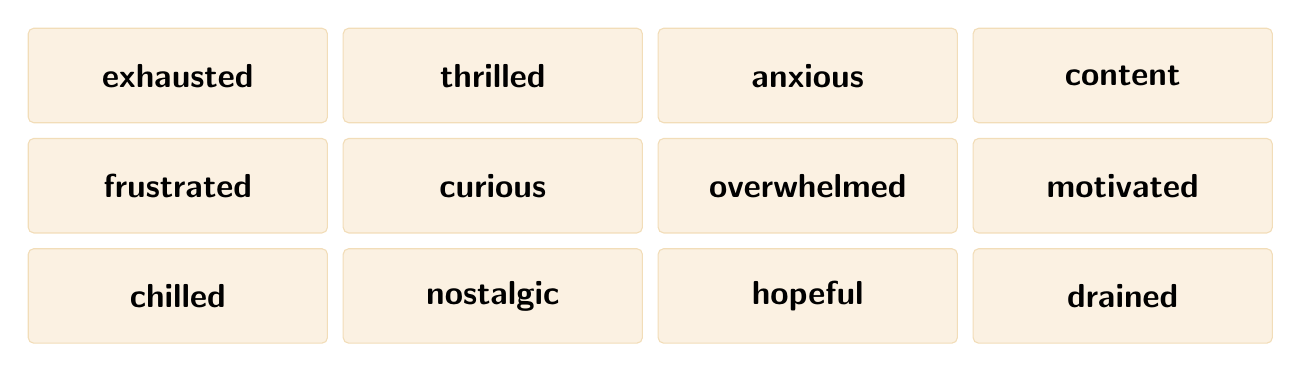
\begin{tikzpicture}[every node/.style={draw=skintintmid,fill=skintint,rounded corners=2pt,minimum width=38mm,minimum height=12mm,font=\fontsize{12}{14}\selectfont\bfseries,align=center,inner sep=2pt}]
    \foreach \lab/\r/\c in {%
      exhausted/0/0, thrilled/0/1, anxious/0/2, content/0/3,
      frustrated/1/0, curious/1/1, overwhelmed/1/2, motivated/1/3,
      chilled/2/0, nostalgic/2/1, hopeful/2/2, drained/2/3%
    } {
      \node at ({\c*4.0},{-\r*1.4}) {\lab};
    }
  \end{tikzpicture}
  \end{center}
}

\begin{document}

% ─────────────────────── COVER ───────────────────────

\thispagestyle{empty}
\vspace*{8mm}
\begin{center}
\includegraphics[height=20mm]{/tmp/somerset-logo.png}\\[10mm]
{\fontsize{12}{14}\selectfont\textcolor{skindeep}{\textsc{Somerset Language Centre · Valencia}}}\\[4mm]
{\fontsize{14}{17}\selectfont\textcolor{somergrey}{Friday Teenagers · 2026–27 · Year 1 of 2}}\\[20mm]
{\fontsize{38}{44}\selectfont\bfseries\textcolor{somerink}{Friday 1}}\\[2mm]
{\fontsize{18}{22}\selectfont\textcolor{skindeep}{18 September 2026}}\\[18mm]
{\fontsize{60}{60}\selectfont\bfseries\textcolor{skinprim}{Jump for joy.}}\\[8mm]
{\fontsize{14}{17}\selectfont\textcolor{somergrey}{\itshape Year opener~ · ~how do you feel about being you?}}\\[14mm]

\begin{tcolorbox}[colback=skintint,colframe=skintintmid,arc=2mm,boxsep=4pt,left=14pt,right=14pt,top=10pt,bottom=10pt,width=0.78\textwidth]
\fontsize{12.5}{16}\selectfont
\textbf{Unit 1 · Close Up B2 (pages 5–16)}\\
Topic: \textbf{emotions \& personality}\\
Grammar: \textbf{present simple vs continuous}\\
FCE focus this Friday: \textbf{Reading Part 5} · \textbf{Listening Part 4} · \textbf{Speaking Part 1}\\
Mandatory extras: short play (Valencia setting) · crossword · wordsearch · false friend \& pronunciation drill
\end{tcolorbox}

\vfill
{\fontsize{11}{13}\selectfont\textcolor{somergrey}{\textit{Read this once before Friday 18 September. ~~ Bring it to class.}}}
\end{center}
\newpage

% ─────────────────────── PAGE 1 — Title + Lead-in + Reading ───────────────────────

\section*{}\sectionmark{F1 — Lead-in \& Reading}
\fridaytitle{Year opener · how do you feel about being you?}{Jump for joy.}{Emotions vocabulary · present simple vs continuous · Aitana's emotional range}

\timelinestrip

\sectionhead{1}{tyextras}{Lead-in — Mood map}{10 min · pairs}{}
\sectionsub{Pick the cell that best describes your week so far. Tell your partner why. Then swap.}
\moodgrid

\sectionhead{2}{tyreading}{Reading — ``Aitana, in four feelings''}{15 min · solo + pair check}{FCE Reading Part 5 (preview)}
\sectionsub{Read the text. Underline every word that describes \textit{how someone feels}.}
\begin{readingbox}
Aitana Oca\~na is one of Spain's biggest pop stars, but she insists she is also \textit{``the most ordinary person in the world.''} She is currently touring the world with \textit{Cuarto Azul}, her fourth album, which came out in May 2025 and won Best Recording Package at the Latin Grammys.

What makes the album interesting isn't the music — it's the \textit{range} of feelings on it. One song is restless and a little anxious. The next is calm, almost shy. A third is thrilled, full of energy. The closing ballad is exhausted and hopeful at the same time.

``I'm always working on something new,'' Aitana told \textit{El Pa\'is} recently. ``Right now I'm writing a song about feeling overwhelmed by being famous. I usually write at night because I think more clearly then. But honestly? Tonight I just want to sleep.''

\pullquote{``I usually write at night because I think more clearly then. But honestly? Tonight I just want to sleep.''}

For her fans in Valencia, the question is simple: which Aitana is performing when she comes to Roig Arena next spring — the thrilled one, the calm one, or the exhausted one? They'll find out together.
\end{readingbox}

\newpage
\section*{}\sectionmark{F1 — Comprehension · Vocabulary · Grammar}

\sectionhead{3}{tyreading}{Comprehension — choose the best answer}{8 min · solo}{FCE Reading Part 5}
\sectionsub{Mirrors the real exam: a long text with multi-choice questions testing detail, opinion, and gist.}
\begin{enumerate}[leftmargin=*]
  \item According to the text, Aitana describes herself as\dots
        \par\hspace{6mm}\textbf{a)} the loudest singer in Spain~\textbf{b)} the most ordinary person in the world~\textbf{c)} the next Rosal\'ia
  \item How many albums has Aitana released so far?
        \par\hspace{6mm}\textbf{a)} two~\textbf{b)} three~\textbf{c)} four
  \item What does the album \textit{Cuarto Azul} show, according to the writer?
        \par\hspace{6mm}\textbf{a)} only happy songs~\textbf{b)} a wide range of feelings~\textbf{c)} songs about Valencia
  \item Why does Aitana usually write at night?
        \par\hspace{6mm}\textbf{a)} her fans demand it~\textbf{b)} she thinks more clearly~\textbf{c)} it's quieter in Madrid
  \item Where will she perform in Valencia?
        \par\hspace{6mm}\textbf{a)} Mestalla~\textbf{b)} Roig Arena~\textbf{c)} Pla\c{c}a de Bous
\end{enumerate}

\sectionhead{4}{tyreading}{Vocabulary — match the feeling word to its meaning}{8 min · pairs}{}
\sectionsub{Definitions are in a different order. Write the matching letter next to each word.}

\begin{tabularx}{\textwidth}{>{\bfseries}l X}
1.~restless     & d) too much to handle right now \\
2.~vulnerable   & a) full of energy and excitement \\
3.~ambitious    & f) easily hurt; not protected emotionally \\
4.~overwhelmed  & b) wanting to succeed; aiming high \\
5.~thrilled     & h) unable to sit still or stop thinking \\
6.~drained      & c) believing things will turn out well \\
7.~hopeful      & g) completely without energy \\
8.~curious      & e) wanting to know or learn more \\
\end{tabularx}

\sectionhead{5}{tygrammar}{Grammar — present simple vs present continuous}{12 min · solo + pair check}{}
\begin{grammarbox}
\textbf{Present simple} = things that are \textit{generally} true, habits, states.\\
\textbf{Present continuous} = things happening \textit{now}, or around now (this week, this month).\\
State verbs (\textit{love, hate, know, believe, want, need}) are almost always simple, even now.\\[3pt]
\textit{Aitana usually writes at night.} ~~vs.~~ \textit{Aitana is writing a song about being famous.}
\end{grammarbox}
\textbf{Choose the correct form. (8 sentences)}
\begin{enumerate}[leftmargin=*]
  \item I \textbf{love / am loving} this song.
  \item Right now Aitana \textbf{tours / is touring} Latin America.
  \item My friend \textbf{thinks / is thinking} Aitana is more interesting than Rosal\'ia.
  \item What \textbf{do you do / are you doing} this weekend?
  \item Pedro \textbf{doesn't know / isn't knowing} the answer.
  \item This week we \textbf{study / are studying} emotions in English class.
  \item Look — that man on the bus \textbf{cries / is crying}!
  \item I \textbf{want / am wanting} to go to the Roig Arena concert.
\end{enumerate}

\newpage
\section*{}\sectionmark{F1 — Speaking · Break · Listening}

\sectionhead{6}{tyspeaking}{Speaking — paired interview}{12 min · pairs (or trios)}{FCE Speaking Part 1}
\sectionsub{In FCE Speaking Part 1, the examiner asks you 4–5 personal questions for about 2 minutes. Today you'll practise being both candidate and examiner with your partner.}
\begin{speakingbox}
\textbf{Format · take turns asking and answering}\\[2pt]
Sit opposite your partner. Take turns. \textbf{Speak in full sentences} — not one-word answers. Use present simple for habits AND present continuous for what's happening now.
\begin{enumerate}[leftmargin=18pt,topsep=4pt]
  \item How are you feeling about the new term so far?
  \item What do you usually do on Friday evenings?
  \item What are you working on outside of school this week?
  \item Tell me about a song or a singer that describes how you feel right now.
  \item Is there something you've never tried that you'd like to?
\end{enumerate}
\end{speakingbox}

\vspace{6pt}
\begin{center}\fontsize{12}{14}\selectfont\textcolor{somergrey}{\textbf{— · — · — ~~ B R E A K ~~ · 5 ~M I N · ~~ — · — · —}}\end{center}

\sectionhead{7}{tylistening}{Listening — How to manage your emotions}{15 min · whole class then solo}{FCE Listening Part 4}
\sectionsub{FCE Listening Part 4 is a 3–4 minute conversation or talk with 6 multi-choice questions, each with 3 options. Today: a 5-minute TED-Ed talk on how to identify, understand and manage emotions. \textbf{You will hear it twice}, just like in the real exam.}
\begin{listeningbox}
\textbf{$\blacktriangleright$ TED-Ed: ``How to manage your emotions''}\\[3pt]
{\fontsize{11.5}{14}\selectfont
Length: 5:09 · narrator + animated illustration · B2-level English\\
YouTube: \href{https://www.youtube.com/watch?v=Uew5BbvmLks}{youtube.com/watch?v=Uew5BbvmLks}\\
TED-Ed: \href{https://ed.ted.com/lessons/how-to-manage-your-emotions}{ed.ted.com/lessons/how-to-manage-your-emotions}}\\[6pt]
\textbf{Before you listen:} read the questions silently (1 min). \textbf{First listen:} mark your best answers. \textbf{Second listen:} check, change, complete.\\[4pt]
\begin{enumerate}[leftmargin=18pt,topsep=2pt]
  \item What is the speaker's main point about emotions?
        \par\hspace{4mm}\textbf{A} They are signals that should always be acted on immediately.
        \par\hspace{4mm}\textbf{B} They are useful information that we can learn to interpret.
        \par\hspace{4mm}\textbf{C} They are obstacles that need to be overcome.
  \item According to the speaker, the first step in managing an emotion is to\dots
        \par\hspace{4mm}\textbf{A} distract yourself from it.
        \par\hspace{4mm}\textbf{B} name what you are feeling.
        \par\hspace{4mm}\textbf{C} ask someone for advice.
  \item The speaker uses the example of a low exam grade in order to\dots
        \par\hspace{4mm}\textbf{A} illustrate how thoughts and feelings interact.
        \par\hspace{4mm}\textbf{B} argue that exams are not a fair measure of ability.
        \par\hspace{4mm}\textbf{C} show that some emotions cannot be changed.
  \item The speaker's attitude towards suppressing emotions is\dots
        \par\hspace{4mm}\textbf{A} strongly opposed.
        \par\hspace{4mm}\textbf{B} generally supportive in moderation.
        \par\hspace{4mm}\textbf{C} neutral — it depends on the situation.
  \item What does the speaker suggest about reframing a difficult feeling?
        \par\hspace{4mm}\textbf{A} It removes the feeling completely.
        \par\hspace{4mm}\textbf{B} It changes the meaning we give the feeling.
        \par\hspace{4mm}\textbf{C} It only works for very mild emotions.
  \item The speaker concludes that emotional skills are\dots
        \par\hspace{4mm}\textbf{A} something we are born with and cannot improve.
        \par\hspace{4mm}\textbf{B} only useful in academic settings.
        \par\hspace{4mm}\textbf{C} a learnable skill that improves with practice.
\end{enumerate}
\end{listeningbox}

\newpage
\section*{}\sectionmark{F1 — Short play \& performance}

\sectionhead{8}{tyspeaking}{Speaking — compare two photos}{8 min · pairs}{FCE Speaking Part 2 (preview)}
\sectionsub{In FCE Speaking Part 2 you're shown two photos and asked to \textbf{compare them} for one minute, then your partner gives a 30-second response. Today is a gentle preview at half-length.}

\begin{speakingbox}
\textbf{Photo A —} a crowd at a concert, hands raised under stage lights (extroverted, social, energetic).\\
\textbf{Photo B —} a person reading quietly at a wooden table (introverted, reflective, calm).\\[6pt]

\textbf{Student A · 60 seconds.}~ Compare the two photos. Which person \textbf{seems more like you}, and why? Use vocabulary from today's reading: \textit{thrilled, restless, content, drained, curious, hopeful}.\\[4pt]
\textbf{Student B · 30 seconds.}~ Tell your partner: which moment have \textbf{you} enjoyed more recently — a busy social moment like Photo A, or a quiet one like Photo B? Why?
\end{speakingbox}

\sectionhead{9}{tyextras}{Short play — ``Outside L'Oceanogr\`afic''}{10 min · pairs}{}
\sectionsub{Read in pairs. One of you is \textbf{Marta}, the other is \textbf{Luc\'ia}. Then swap roles.}
\begin{playbox}
\textit{Setting: Outside the entrance to L'Oceanogr\`afic, Valencia. A Friday afternoon in mid-September. The first weekend after school has started.}\\[6pt]
\textbf{MARTA:} Luc\'ia! What are you doing here? I thought you were studying this weekend.\\[2pt]
\textbf{LUC\'IA:} I am — I mean, I'm supposed to be. But honestly, I'm feeling a bit overwhelmed. My brother brought me to see the dolphins.\\[2pt]
\textbf{MARTA:} The dolphins fix everything. How's the new term going?\\[2pt]
\textbf{LUC\'IA:} It's OK. I love my English class — we're reading about Aitana this week. But maths? I don't even understand the homework.\\[2pt]
\textbf{MARTA:} Same. Every September I think I'm going to be different. Then by Tuesday I'm exhausted again.\\[2pt]
\textbf{LUC\'IA:} Are you free tomorrow? I'm going to Malvarrosa with some friends.\\[2pt]
\textbf{MARTA:} Tomorrow I'm visiting my grandmother in Albacete. But Sunday — yes!\\[2pt]
\textbf{LUC\'IA:} Good. Right now I just want a horchata. Want one?\\[2pt]
\textbf{MARTA:} Always.
\nowperform
\end{playbox}

\sectionhead{10}{tyspeaking}{Speaking 2 — ``What are you up to?'' info-gap}{12 min · pairs OR trios (cards at back)}{}
\sectionsub{Your teacher will give you a card from the back of the booklet. \textbf{Don't show your partner.} You have a fictional life this week — tell your partner about it, ask about theirs. Use \textit{present simple} for habits, \textit{present continuous} for what's happening now.}
\begin{speakingbox}
\textbf{Stages}
\begin{enumerate}[leftmargin=18pt,topsep=2pt]
  \item \textbf{2 min planning.} Read your card silently. Plan what you'll say.
  \item \textbf{7 min interview.} Find out about your partner. Take notes.
  \item \textbf{3 min report.} Tell the class one interesting thing about your partner's week.
\end{enumerate}
\end{speakingbox}

\newpage
\section*{}\sectionmark{F1 — Crossword (student)}
\sectionhead{11}{tyextras}{Crossword — emotion adjectives}{8 min · solo or pairs}{}
\sectionsub{Use the clues to fill in the grid. Letters in shared cells will help you check.}

\begin{center}
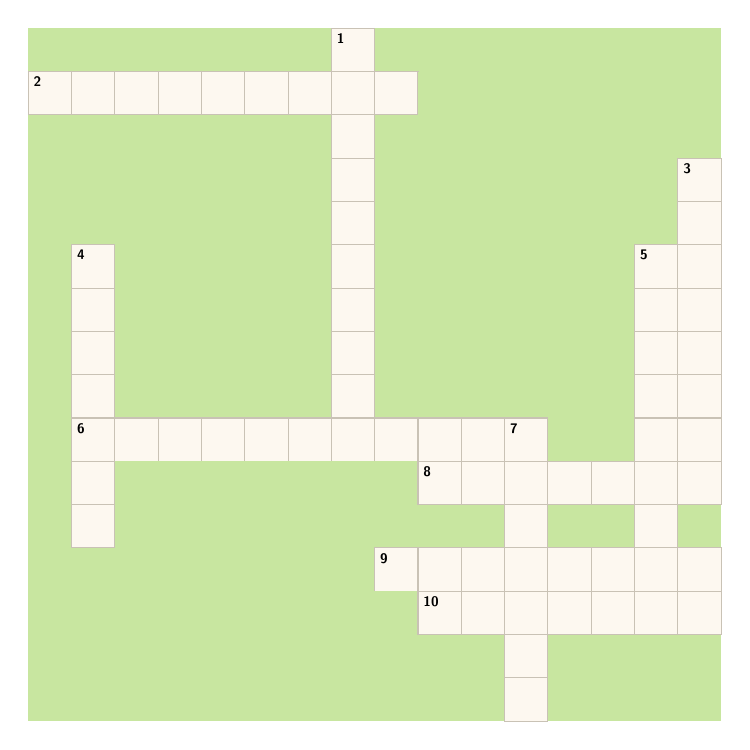
\begin{tikzpicture}[x=0.55cm,y=0.55cm]
\fill[deadcell] (0,0) rectangle (1,-1);
\fill[deadcell] (1,0) rectangle (2,-1);
\fill[deadcell] (2,0) rectangle (3,-1);
\fill[deadcell] (3,0) rectangle (4,-1);
\fill[deadcell] (4,0) rectangle (5,-1);
\fill[deadcell] (5,0) rectangle (6,-1);
\fill[deadcell] (6,0) rectangle (7,-1);
\fill[livecell] (7,0) rectangle (8,-1);
\draw[livecellborder] (7,0) rectangle (8,-1);
\node[anchor=north west,font=\tiny\bfseries,inner sep=1pt] at (7.05,-0.05) {1};
\fill[deadcell] (8,0) rectangle (9,-1);
\fill[deadcell] (9,0) rectangle (10,-1);
\fill[deadcell] (10,0) rectangle (11,-1);
\fill[deadcell] (11,0) rectangle (12,-1);
\fill[deadcell] (12,0) rectangle (13,-1);
\fill[deadcell] (13,0) rectangle (14,-1);
\fill[deadcell] (14,0) rectangle (15,-1);
\fill[deadcell] (15,0) rectangle (16,-1);
\fill[livecell] (0,-1) rectangle (1,-2);
\draw[livecellborder] (0,-1) rectangle (1,-2);
\node[anchor=north west,font=\tiny\bfseries,inner sep=1pt] at (0.05,-1.05) {2};
\fill[livecell] (1,-1) rectangle (2,-2);
\draw[livecellborder] (1,-1) rectangle (2,-2);
\fill[livecell] (2,-1) rectangle (3,-2);
\draw[livecellborder] (2,-1) rectangle (3,-2);
\fill[livecell] (3,-1) rectangle (4,-2);
\draw[livecellborder] (3,-1) rectangle (4,-2);
\fill[livecell] (4,-1) rectangle (5,-2);
\draw[livecellborder] (4,-1) rectangle (5,-2);
\fill[livecell] (5,-1) rectangle (6,-2);
\draw[livecellborder] (5,-1) rectangle (6,-2);
\fill[livecell] (6,-1) rectangle (7,-2);
\draw[livecellborder] (6,-1) rectangle (7,-2);
\fill[livecell] (7,-1) rectangle (8,-2);
\draw[livecellborder] (7,-1) rectangle (8,-2);
\fill[livecell] (8,-1) rectangle (9,-2);
\draw[livecellborder] (8,-1) rectangle (9,-2);
\fill[deadcell] (9,-1) rectangle (10,-2);
\fill[deadcell] (10,-1) rectangle (11,-2);
\fill[deadcell] (11,-1) rectangle (12,-2);
\fill[deadcell] (12,-1) rectangle (13,-2);
\fill[deadcell] (13,-1) rectangle (14,-2);
\fill[deadcell] (14,-1) rectangle (15,-2);
\fill[deadcell] (15,-1) rectangle (16,-2);
\fill[deadcell] (0,-2) rectangle (1,-3);
\fill[deadcell] (1,-2) rectangle (2,-3);
\fill[deadcell] (2,-2) rectangle (3,-3);
\fill[deadcell] (3,-2) rectangle (4,-3);
\fill[deadcell] (4,-2) rectangle (5,-3);
\fill[deadcell] (5,-2) rectangle (6,-3);
\fill[deadcell] (6,-2) rectangle (7,-3);
\fill[livecell] (7,-2) rectangle (8,-3);
\draw[livecellborder] (7,-2) rectangle (8,-3);
\fill[deadcell] (8,-2) rectangle (9,-3);
\fill[deadcell] (9,-2) rectangle (10,-3);
\fill[deadcell] (10,-2) rectangle (11,-3);
\fill[deadcell] (11,-2) rectangle (12,-3);
\fill[deadcell] (12,-2) rectangle (13,-3);
\fill[deadcell] (13,-2) rectangle (14,-3);
\fill[deadcell] (14,-2) rectangle (15,-3);
\fill[deadcell] (15,-2) rectangle (16,-3);
\fill[deadcell] (0,-3) rectangle (1,-4);
\fill[deadcell] (1,-3) rectangle (2,-4);
\fill[deadcell] (2,-3) rectangle (3,-4);
\fill[deadcell] (3,-3) rectangle (4,-4);
\fill[deadcell] (4,-3) rectangle (5,-4);
\fill[deadcell] (5,-3) rectangle (6,-4);
\fill[deadcell] (6,-3) rectangle (7,-4);
\fill[livecell] (7,-3) rectangle (8,-4);
\draw[livecellborder] (7,-3) rectangle (8,-4);
\fill[deadcell] (8,-3) rectangle (9,-4);
\fill[deadcell] (9,-3) rectangle (10,-4);
\fill[deadcell] (10,-3) rectangle (11,-4);
\fill[deadcell] (11,-3) rectangle (12,-4);
\fill[deadcell] (12,-3) rectangle (13,-4);
\fill[deadcell] (13,-3) rectangle (14,-4);
\fill[deadcell] (14,-3) rectangle (15,-4);
\fill[livecell] (15,-3) rectangle (16,-4);
\draw[livecellborder] (15,-3) rectangle (16,-4);
\node[anchor=north west,font=\tiny\bfseries,inner sep=1pt] at (15.05,-3.05) {3};
\fill[deadcell] (0,-4) rectangle (1,-5);
\fill[deadcell] (1,-4) rectangle (2,-5);
\fill[deadcell] (2,-4) rectangle (3,-5);
\fill[deadcell] (3,-4) rectangle (4,-5);
\fill[deadcell] (4,-4) rectangle (5,-5);
\fill[deadcell] (5,-4) rectangle (6,-5);
\fill[deadcell] (6,-4) rectangle (7,-5);
\fill[livecell] (7,-4) rectangle (8,-5);
\draw[livecellborder] (7,-4) rectangle (8,-5);
\fill[deadcell] (8,-4) rectangle (9,-5);
\fill[deadcell] (9,-4) rectangle (10,-5);
\fill[deadcell] (10,-4) rectangle (11,-5);
\fill[deadcell] (11,-4) rectangle (12,-5);
\fill[deadcell] (12,-4) rectangle (13,-5);
\fill[deadcell] (13,-4) rectangle (14,-5);
\fill[deadcell] (14,-4) rectangle (15,-5);
\fill[livecell] (15,-4) rectangle (16,-5);
\draw[livecellborder] (15,-4) rectangle (16,-5);
\fill[deadcell] (0,-5) rectangle (1,-6);
\fill[livecell] (1,-5) rectangle (2,-6);
\draw[livecellborder] (1,-5) rectangle (2,-6);
\node[anchor=north west,font=\tiny\bfseries,inner sep=1pt] at (1.05,-5.05) {4};
\fill[deadcell] (2,-5) rectangle (3,-6);
\fill[deadcell] (3,-5) rectangle (4,-6);
\fill[deadcell] (4,-5) rectangle (5,-6);
\fill[deadcell] (5,-5) rectangle (6,-6);
\fill[deadcell] (6,-5) rectangle (7,-6);
\fill[livecell] (7,-5) rectangle (8,-6);
\draw[livecellborder] (7,-5) rectangle (8,-6);
\fill[deadcell] (8,-5) rectangle (9,-6);
\fill[deadcell] (9,-5) rectangle (10,-6);
\fill[deadcell] (10,-5) rectangle (11,-6);
\fill[deadcell] (11,-5) rectangle (12,-6);
\fill[deadcell] (12,-5) rectangle (13,-6);
\fill[deadcell] (13,-5) rectangle (14,-6);
\fill[livecell] (14,-5) rectangle (15,-6);
\draw[livecellborder] (14,-5) rectangle (15,-6);
\node[anchor=north west,font=\tiny\bfseries,inner sep=1pt] at (14.05,-5.05) {5};
\fill[livecell] (15,-5) rectangle (16,-6);
\draw[livecellborder] (15,-5) rectangle (16,-6);
\fill[deadcell] (0,-6) rectangle (1,-7);
\fill[livecell] (1,-6) rectangle (2,-7);
\draw[livecellborder] (1,-6) rectangle (2,-7);
\fill[deadcell] (2,-6) rectangle (3,-7);
\fill[deadcell] (3,-6) rectangle (4,-7);
\fill[deadcell] (4,-6) rectangle (5,-7);
\fill[deadcell] (5,-6) rectangle (6,-7);
\fill[deadcell] (6,-6) rectangle (7,-7);
\fill[livecell] (7,-6) rectangle (8,-7);
\draw[livecellborder] (7,-6) rectangle (8,-7);
\fill[deadcell] (8,-6) rectangle (9,-7);
\fill[deadcell] (9,-6) rectangle (10,-7);
\fill[deadcell] (10,-6) rectangle (11,-7);
\fill[deadcell] (11,-6) rectangle (12,-7);
\fill[deadcell] (12,-6) rectangle (13,-7);
\fill[deadcell] (13,-6) rectangle (14,-7);
\fill[livecell] (14,-6) rectangle (15,-7);
\draw[livecellborder] (14,-6) rectangle (15,-7);
\fill[livecell] (15,-6) rectangle (16,-7);
\draw[livecellborder] (15,-6) rectangle (16,-7);
\fill[deadcell] (0,-7) rectangle (1,-8);
\fill[livecell] (1,-7) rectangle (2,-8);
\draw[livecellborder] (1,-7) rectangle (2,-8);
\fill[deadcell] (2,-7) rectangle (3,-8);
\fill[deadcell] (3,-7) rectangle (4,-8);
\fill[deadcell] (4,-7) rectangle (5,-8);
\fill[deadcell] (5,-7) rectangle (6,-8);
\fill[deadcell] (6,-7) rectangle (7,-8);
\fill[livecell] (7,-7) rectangle (8,-8);
\draw[livecellborder] (7,-7) rectangle (8,-8);
\fill[deadcell] (8,-7) rectangle (9,-8);
\fill[deadcell] (9,-7) rectangle (10,-8);
\fill[deadcell] (10,-7) rectangle (11,-8);
\fill[deadcell] (11,-7) rectangle (12,-8);
\fill[deadcell] (12,-7) rectangle (13,-8);
\fill[deadcell] (13,-7) rectangle (14,-8);
\fill[livecell] (14,-7) rectangle (15,-8);
\draw[livecellborder] (14,-7) rectangle (15,-8);
\fill[livecell] (15,-7) rectangle (16,-8);
\draw[livecellborder] (15,-7) rectangle (16,-8);
\fill[deadcell] (0,-8) rectangle (1,-9);
\fill[livecell] (1,-8) rectangle (2,-9);
\draw[livecellborder] (1,-8) rectangle (2,-9);
\fill[deadcell] (2,-8) rectangle (3,-9);
\fill[deadcell] (3,-8) rectangle (4,-9);
\fill[deadcell] (4,-8) rectangle (5,-9);
\fill[deadcell] (5,-8) rectangle (6,-9);
\fill[deadcell] (6,-8) rectangle (7,-9);
\fill[livecell] (7,-8) rectangle (8,-9);
\draw[livecellborder] (7,-8) rectangle (8,-9);
\fill[deadcell] (8,-8) rectangle (9,-9);
\fill[deadcell] (9,-8) rectangle (10,-9);
\fill[deadcell] (10,-8) rectangle (11,-9);
\fill[deadcell] (11,-8) rectangle (12,-9);
\fill[deadcell] (12,-8) rectangle (13,-9);
\fill[deadcell] (13,-8) rectangle (14,-9);
\fill[livecell] (14,-8) rectangle (15,-9);
\draw[livecellborder] (14,-8) rectangle (15,-9);
\fill[livecell] (15,-8) rectangle (16,-9);
\draw[livecellborder] (15,-8) rectangle (16,-9);
\fill[deadcell] (0,-9) rectangle (1,-10);
\fill[livecell] (1,-9) rectangle (2,-10);
\draw[livecellborder] (1,-9) rectangle (2,-10);
\node[anchor=north west,font=\tiny\bfseries,inner sep=1pt] at (1.05,-9.05) {6};
\fill[livecell] (2,-9) rectangle (3,-10);
\draw[livecellborder] (2,-9) rectangle (3,-10);
\fill[livecell] (3,-9) rectangle (4,-10);
\draw[livecellborder] (3,-9) rectangle (4,-10);
\fill[livecell] (4,-9) rectangle (5,-10);
\draw[livecellborder] (4,-9) rectangle (5,-10);
\fill[livecell] (5,-9) rectangle (6,-10);
\draw[livecellborder] (5,-9) rectangle (6,-10);
\fill[livecell] (6,-9) rectangle (7,-10);
\draw[livecellborder] (6,-9) rectangle (7,-10);
\fill[livecell] (7,-9) rectangle (8,-10);
\draw[livecellborder] (7,-9) rectangle (8,-10);
\fill[livecell] (8,-9) rectangle (9,-10);
\draw[livecellborder] (8,-9) rectangle (9,-10);
\fill[livecell] (9,-9) rectangle (10,-10);
\draw[livecellborder] (9,-9) rectangle (10,-10);
\fill[livecell] (10,-9) rectangle (11,-10);
\draw[livecellborder] (10,-9) rectangle (11,-10);
\fill[livecell] (11,-9) rectangle (12,-10);
\draw[livecellborder] (11,-9) rectangle (12,-10);
\node[anchor=north west,font=\tiny\bfseries,inner sep=1pt] at (11.05,-9.05) {7};
\fill[deadcell] (12,-9) rectangle (13,-10);
\fill[deadcell] (13,-9) rectangle (14,-10);
\fill[livecell] (14,-9) rectangle (15,-10);
\draw[livecellborder] (14,-9) rectangle (15,-10);
\fill[livecell] (15,-9) rectangle (16,-10);
\draw[livecellborder] (15,-9) rectangle (16,-10);
\fill[deadcell] (0,-10) rectangle (1,-11);
\fill[livecell] (1,-10) rectangle (2,-11);
\draw[livecellborder] (1,-10) rectangle (2,-11);
\fill[deadcell] (2,-10) rectangle (3,-11);
\fill[deadcell] (3,-10) rectangle (4,-11);
\fill[deadcell] (4,-10) rectangle (5,-11);
\fill[deadcell] (5,-10) rectangle (6,-11);
\fill[deadcell] (6,-10) rectangle (7,-11);
\fill[deadcell] (7,-10) rectangle (8,-11);
\fill[deadcell] (8,-10) rectangle (9,-11);
\fill[livecell] (9,-10) rectangle (10,-11);
\draw[livecellborder] (9,-10) rectangle (10,-11);
\node[anchor=north west,font=\tiny\bfseries,inner sep=1pt] at (9.05,-10.05) {8};
\fill[livecell] (10,-10) rectangle (11,-11);
\draw[livecellborder] (10,-10) rectangle (11,-11);
\fill[livecell] (11,-10) rectangle (12,-11);
\draw[livecellborder] (11,-10) rectangle (12,-11);
\fill[livecell] (12,-10) rectangle (13,-11);
\draw[livecellborder] (12,-10) rectangle (13,-11);
\fill[livecell] (13,-10) rectangle (14,-11);
\draw[livecellborder] (13,-10) rectangle (14,-11);
\fill[livecell] (14,-10) rectangle (15,-11);
\draw[livecellborder] (14,-10) rectangle (15,-11);
\fill[livecell] (15,-10) rectangle (16,-11);
\draw[livecellborder] (15,-10) rectangle (16,-11);
\fill[deadcell] (0,-11) rectangle (1,-12);
\fill[livecell] (1,-11) rectangle (2,-12);
\draw[livecellborder] (1,-11) rectangle (2,-12);
\fill[deadcell] (2,-11) rectangle (3,-12);
\fill[deadcell] (3,-11) rectangle (4,-12);
\fill[deadcell] (4,-11) rectangle (5,-12);
\fill[deadcell] (5,-11) rectangle (6,-12);
\fill[deadcell] (6,-11) rectangle (7,-12);
\fill[deadcell] (7,-11) rectangle (8,-12);
\fill[deadcell] (8,-11) rectangle (9,-12);
\fill[deadcell] (9,-11) rectangle (10,-12);
\fill[deadcell] (10,-11) rectangle (11,-12);
\fill[livecell] (11,-11) rectangle (12,-12);
\draw[livecellborder] (11,-11) rectangle (12,-12);
\fill[deadcell] (12,-11) rectangle (13,-12);
\fill[deadcell] (13,-11) rectangle (14,-12);
\fill[livecell] (14,-11) rectangle (15,-12);
\draw[livecellborder] (14,-11) rectangle (15,-12);
\fill[deadcell] (15,-11) rectangle (16,-12);
\fill[deadcell] (0,-12) rectangle (1,-13);
\fill[deadcell] (1,-12) rectangle (2,-13);
\fill[deadcell] (2,-12) rectangle (3,-13);
\fill[deadcell] (3,-12) rectangle (4,-13);
\fill[deadcell] (4,-12) rectangle (5,-13);
\fill[deadcell] (5,-12) rectangle (6,-13);
\fill[deadcell] (6,-12) rectangle (7,-13);
\fill[deadcell] (7,-12) rectangle (8,-13);
\fill[livecell] (8,-12) rectangle (9,-13);
\draw[livecellborder] (8,-12) rectangle (9,-13);
\node[anchor=north west,font=\tiny\bfseries,inner sep=1pt] at (8.05,-12.05) {9};
\fill[livecell] (9,-12) rectangle (10,-13);
\draw[livecellborder] (9,-12) rectangle (10,-13);
\fill[livecell] (10,-12) rectangle (11,-13);
\draw[livecellborder] (10,-12) rectangle (11,-13);
\fill[livecell] (11,-12) rectangle (12,-13);
\draw[livecellborder] (11,-12) rectangle (12,-13);
\fill[livecell] (12,-12) rectangle (13,-13);
\draw[livecellborder] (12,-12) rectangle (13,-13);
\fill[livecell] (13,-12) rectangle (14,-13);
\draw[livecellborder] (13,-12) rectangle (14,-13);
\fill[livecell] (14,-12) rectangle (15,-13);
\draw[livecellborder] (14,-12) rectangle (15,-13);
\fill[livecell] (15,-12) rectangle (16,-13);
\draw[livecellborder] (15,-12) rectangle (16,-13);
\fill[deadcell] (0,-13) rectangle (1,-14);
\fill[deadcell] (1,-13) rectangle (2,-14);
\fill[deadcell] (2,-13) rectangle (3,-14);
\fill[deadcell] (3,-13) rectangle (4,-14);
\fill[deadcell] (4,-13) rectangle (5,-14);
\fill[deadcell] (5,-13) rectangle (6,-14);
\fill[deadcell] (6,-13) rectangle (7,-14);
\fill[deadcell] (7,-13) rectangle (8,-14);
\fill[deadcell] (8,-13) rectangle (9,-14);
\fill[livecell] (9,-13) rectangle (10,-14);
\draw[livecellborder] (9,-13) rectangle (10,-14);
\node[anchor=north west,font=\tiny\bfseries,inner sep=1pt] at (9.05,-13.05) {10};
\fill[livecell] (10,-13) rectangle (11,-14);
\draw[livecellborder] (10,-13) rectangle (11,-14);
\fill[livecell] (11,-13) rectangle (12,-14);
\draw[livecellborder] (11,-13) rectangle (12,-14);
\fill[livecell] (12,-13) rectangle (13,-14);
\draw[livecellborder] (12,-13) rectangle (13,-14);
\fill[livecell] (13,-13) rectangle (14,-14);
\draw[livecellborder] (13,-13) rectangle (14,-14);
\fill[livecell] (14,-13) rectangle (15,-14);
\draw[livecellborder] (14,-13) rectangle (15,-14);
\fill[livecell] (15,-13) rectangle (16,-14);
\draw[livecellborder] (15,-13) rectangle (16,-14);
\fill[deadcell] (0,-14) rectangle (1,-15);
\fill[deadcell] (1,-14) rectangle (2,-15);
\fill[deadcell] (2,-14) rectangle (3,-15);
\fill[deadcell] (3,-14) rectangle (4,-15);
\fill[deadcell] (4,-14) rectangle (5,-15);
\fill[deadcell] (5,-14) rectangle (6,-15);
\fill[deadcell] (6,-14) rectangle (7,-15);
\fill[deadcell] (7,-14) rectangle (8,-15);
\fill[deadcell] (8,-14) rectangle (9,-15);
\fill[deadcell] (9,-14) rectangle (10,-15);
\fill[deadcell] (10,-14) rectangle (11,-15);
\fill[livecell] (11,-14) rectangle (12,-15);
\draw[livecellborder] (11,-14) rectangle (12,-15);
\fill[deadcell] (12,-14) rectangle (13,-15);
\fill[deadcell] (13,-14) rectangle (14,-15);
\fill[deadcell] (14,-14) rectangle (15,-15);
\fill[deadcell] (15,-14) rectangle (16,-15);
\fill[deadcell] (0,-15) rectangle (1,-16);
\fill[deadcell] (1,-15) rectangle (2,-16);
\fill[deadcell] (2,-15) rectangle (3,-16);
\fill[deadcell] (3,-15) rectangle (4,-16);
\fill[deadcell] (4,-15) rectangle (5,-16);
\fill[deadcell] (5,-15) rectangle (6,-16);
\fill[deadcell] (6,-15) rectangle (7,-16);
\fill[deadcell] (7,-15) rectangle (8,-16);
\fill[deadcell] (8,-15) rectangle (9,-16);
\fill[deadcell] (9,-15) rectangle (10,-16);
\fill[deadcell] (10,-15) rectangle (11,-16);
\fill[livecell] (11,-15) rectangle (12,-16);
\draw[livecellborder] (11,-15) rectangle (12,-16);
\fill[deadcell] (12,-15) rectangle (13,-16);
\fill[deadcell] (13,-15) rectangle (14,-16);
\fill[deadcell] (14,-15) rectangle (15,-16);
\fill[deadcell] (15,-15) rectangle (16,-16);
\end{tikzpicture}
\end{center}

\vspace{6pt}
\begin{multicols}{2}
{\fontsize{12}{15}\selectfont
\textbf{\textcolor{tyreading}{Across}}\\[2pt]
\textbf{2} (9) — wanting strongly to succeed in life \\
\textbf{6} (11) — feeling that you have too much to handle \\
\textbf{8} (7) — wanting to know or learn more \\
\textbf{9} (8) — extremely excited and pleased \\
\textbf{10} (7) — quietly happy with how things are \\
\columnbreak
\textbf{\textcolor{tygrammar}{Down}}\\[2pt]
\textbf{1} (10) — easily hurt; not protected emotionally \\
\textbf{3} (8) — unable to sit still or stop thinking \\
\textbf{4} (7) — worried or nervous about something \\
\textbf{5} (7) — believing things will turn out well \\
\textbf{7} (7) — completely without energy after effort \\
}
\end{multicols}

\newpage
\section*{}\sectionmark{F1 — Wordsearch (student)}
\sectionhead{12}{tyextras}{Wordsearch — find from the clues}{6 min · solo}{}
\sectionsub{Read the clue, work out the word, then find it in the grid. Words go horizontally, vertically and diagonally — forwards or backwards. One clue refers to Valencia.}

\begin{center}

\begin{tikzpicture}[x=0.55cm,y=0.55cm]
\fill[livecell] (0,0) rectangle (1,-1);
\draw[livecellborder] (0,0) rectangle (1,-1);
\node[font=\bfseries] at (0.5,-0.55) {K};
\fill[livecell] (1,0) rectangle (2,-1);
\draw[livecellborder] (1,0) rectangle (2,-1);
\node[font=\bfseries] at (1.5,-0.55) {C};
\fill[livecell] (2,0) rectangle (3,-1);
\draw[livecellborder] (2,0) rectangle (3,-1);
\node[font=\bfseries] at (2.5,-0.55) {O};
\fill[livecell] (3,0) rectangle (4,-1);
\draw[livecellborder] (3,0) rectangle (4,-1);
\node[font=\bfseries] at (3.5,-0.55) {N};
\fill[livecell] (4,0) rectangle (5,-1);
\draw[livecellborder] (4,0) rectangle (5,-1);
\node[font=\bfseries] at (4.5,-0.55) {T};
\fill[livecell] (5,0) rectangle (6,-1);
\draw[livecellborder] (5,0) rectangle (6,-1);
\node[font=\bfseries] at (5.5,-0.55) {E};
\fill[livecell] (6,0) rectangle (7,-1);
\draw[livecellborder] (6,0) rectangle (7,-1);
\node[font=\bfseries] at (6.5,-0.55) {N};
\fill[livecell] (7,0) rectangle (8,-1);
\draw[livecellborder] (7,0) rectangle (8,-1);
\node[font=\bfseries] at (7.5,-0.55) {T};
\fill[livecell] (8,0) rectangle (9,-1);
\draw[livecellborder] (8,0) rectangle (9,-1);
\node[font=\bfseries] at (8.5,-0.55) {E};
\fill[livecell] (9,0) rectangle (10,-1);
\draw[livecellborder] (9,0) rectangle (10,-1);
\node[font=\bfseries] at (9.5,-0.55) {M};
\fill[livecell] (10,0) rectangle (11,-1);
\draw[livecellborder] (10,0) rectangle (11,-1);
\node[font=\bfseries] at (10.5,-0.55) {U};
\fill[livecell] (11,0) rectangle (12,-1);
\draw[livecellborder] (11,0) rectangle (12,-1);
\node[font=\bfseries] at (11.5,-0.55) {B};
\fill[livecell] (0,-1) rectangle (1,-2);
\draw[livecellborder] (0,-1) rectangle (1,-2);
\node[font=\bfseries] at (0.5,-1.55) {D};
\fill[livecell] (1,-1) rectangle (2,-2);
\draw[livecellborder] (1,-1) rectangle (2,-2);
\node[font=\bfseries] at (1.5,-1.55) {E};
\fill[livecell] (2,-1) rectangle (3,-2);
\draw[livecellborder] (2,-1) rectangle (3,-2);
\node[font=\bfseries] at (2.5,-1.55) {N};
\fill[livecell] (3,-1) rectangle (4,-2);
\draw[livecellborder] (3,-1) rectangle (4,-2);
\node[font=\bfseries] at (3.5,-1.55) {I};
\fill[livecell] (4,-1) rectangle (5,-2);
\draw[livecellborder] (4,-1) rectangle (5,-2);
\node[font=\bfseries] at (4.5,-1.55) {A};
\fill[livecell] (5,-1) rectangle (6,-2);
\draw[livecellborder] (5,-1) rectangle (6,-2);
\node[font=\bfseries] at (5.5,-1.55) {R};
\fill[livecell] (6,-1) rectangle (7,-2);
\draw[livecellborder] (6,-1) rectangle (7,-2);
\node[font=\bfseries] at (6.5,-1.55) {D};
\fill[livecell] (7,-1) rectangle (8,-2);
\draw[livecellborder] (7,-1) rectangle (8,-2);
\node[font=\bfseries] at (7.5,-1.55) {C};
\fill[livecell] (8,-1) rectangle (9,-2);
\draw[livecellborder] (8,-1) rectangle (9,-2);
\node[font=\bfseries] at (8.5,-1.55) {R};
\fill[livecell] (9,-1) rectangle (10,-2);
\draw[livecellborder] (9,-1) rectangle (10,-2);
\node[font=\bfseries] at (9.5,-1.55) {A};
\fill[livecell] (10,-1) rectangle (11,-2);
\draw[livecellborder] (10,-1) rectangle (11,-2);
\node[font=\bfseries] at (10.5,-1.55) {D};
\fill[livecell] (11,-1) rectangle (12,-2);
\draw[livecellborder] (11,-1) rectangle (12,-2);
\node[font=\bfseries] at (11.5,-1.55) {L};
\fill[livecell] (0,-2) rectangle (1,-3);
\draw[livecellborder] (0,-2) rectangle (1,-3);
\node[font=\bfseries] at (0.5,-2.55) {V};
\fill[livecell] (1,-2) rectangle (2,-3);
\draw[livecellborder] (1,-2) rectangle (2,-3);
\node[font=\bfseries] at (1.5,-2.55) {S};
\fill[livecell] (2,-2) rectangle (3,-3);
\draw[livecellborder] (2,-2) rectangle (3,-3);
\node[font=\bfseries] at (2.5,-2.55) {B};
\fill[livecell] (3,-2) rectangle (4,-3);
\draw[livecellborder] (3,-2) rectangle (4,-3);
\node[font=\bfseries] at (3.5,-2.55) {Q};
\fill[livecell] (4,-2) rectangle (5,-3);
\draw[livecellborder] (4,-2) rectangle (5,-3);
\node[font=\bfseries] at (4.5,-2.55) {L};
\fill[livecell] (5,-2) rectangle (6,-3);
\draw[livecellborder] (5,-2) rectangle (6,-3);
\node[font=\bfseries] at (5.5,-2.55) {G};
\fill[livecell] (6,-2) rectangle (7,-3);
\draw[livecellborder] (6,-2) rectangle (7,-3);
\node[font=\bfseries] at (6.5,-2.55) {B};
\fill[livecell] (7,-2) rectangle (8,-3);
\draw[livecellborder] (7,-2) rectangle (8,-3);
\node[font=\bfseries] at (7.5,-2.55) {C};
\fill[livecell] (8,-2) rectangle (9,-3);
\draw[livecellborder] (8,-2) rectangle (9,-3);
\node[font=\bfseries] at (8.5,-2.55) {N};
\fill[livecell] (9,-2) rectangle (10,-3);
\draw[livecellborder] (9,-2) rectangle (10,-3);
\node[font=\bfseries] at (9.5,-2.55) {M};
\fill[livecell] (10,-2) rectangle (11,-3);
\draw[livecellborder] (10,-2) rectangle (11,-3);
\node[font=\bfseries] at (10.5,-2.55) {N};
\fill[livecell] (11,-2) rectangle (12,-3);
\draw[livecellborder] (11,-2) rectangle (12,-3);
\node[font=\bfseries] at (11.5,-2.55) {A};
\fill[livecell] (0,-3) rectangle (1,-4);
\draw[livecellborder] (0,-3) rectangle (1,-4);
\node[font=\bfseries] at (0.5,-3.55) {A};
\fill[livecell] (1,-3) rectangle (2,-4);
\draw[livecellborder] (1,-3) rectangle (2,-4);
\node[font=\bfseries] at (1.5,-3.55) {C};
\fill[livecell] (2,-3) rectangle (3,-4);
\draw[livecellborder] (2,-3) rectangle (3,-4);
\node[font=\bfseries] at (2.5,-3.55) {R};
\fill[livecell] (3,-3) rectangle (4,-4);
\draw[livecellborder] (3,-3) rectangle (4,-4);
\node[font=\bfseries] at (3.5,-3.55) {H};
\fill[livecell] (4,-3) rectangle (5,-4);
\draw[livecellborder] (4,-3) rectangle (5,-4);
\node[font=\bfseries] at (4.5,-3.55) {U};
\fill[livecell] (5,-3) rectangle (6,-4);
\draw[livecellborder] (5,-3) rectangle (6,-4);
\node[font=\bfseries] at (5.5,-3.55) {C};
\fill[livecell] (6,-3) rectangle (7,-4);
\draw[livecellborder] (6,-3) rectangle (7,-4);
\node[font=\bfseries] at (6.5,-3.55) {S};
\fill[livecell] (7,-3) rectangle (8,-4);
\draw[livecellborder] (7,-3) rectangle (8,-4);
\node[font=\bfseries] at (7.5,-3.55) {R};
\fill[livecell] (8,-3) rectangle (9,-4);
\draw[livecellborder] (8,-3) rectangle (9,-4);
\node[font=\bfseries] at (8.5,-3.55) {N};
\fill[livecell] (9,-3) rectangle (10,-4);
\draw[livecellborder] (9,-3) rectangle (10,-4);
\node[font=\bfseries] at (9.5,-3.55) {B};
\fill[livecell] (10,-3) rectangle (11,-4);
\draw[livecellborder] (10,-3) rectangle (11,-4);
\node[font=\bfseries] at (10.5,-3.55) {E};
\fill[livecell] (11,-3) rectangle (12,-4);
\draw[livecellborder] (11,-3) rectangle (12,-4);
\node[font=\bfseries] at (11.5,-3.55) {N};
\fill[livecell] (0,-4) rectangle (1,-5);
\draw[livecellborder] (0,-4) rectangle (1,-5);
\node[font=\bfseries] at (0.5,-4.55) {L};
\fill[livecell] (1,-4) rectangle (2,-5);
\draw[livecellborder] (1,-4) rectangle (2,-5);
\node[font=\bfseries] at (1.5,-4.55) {B};
\fill[livecell] (2,-4) rectangle (3,-5);
\draw[livecellborder] (2,-4) rectangle (3,-5);
\node[font=\bfseries] at (2.5,-4.55) {E};
\fill[livecell] (3,-4) rectangle (4,-5);
\draw[livecellborder] (3,-4) rectangle (4,-5);
\node[font=\bfseries] at (3.5,-4.55) {S};
\fill[livecell] (4,-4) rectangle (5,-5);
\draw[livecellborder] (4,-4) rectangle (5,-5);
\node[font=\bfseries] at (4.5,-4.55) {F};
\fill[livecell] (5,-4) rectangle (6,-5);
\draw[livecellborder] (5,-4) rectangle (6,-5);
\node[font=\bfseries] at (5.5,-4.55) {D};
\fill[livecell] (6,-4) rectangle (7,-5);
\draw[livecellborder] (6,-4) rectangle (7,-5);
\node[font=\bfseries] at (6.5,-4.55) {U};
\fill[livecell] (7,-4) rectangle (8,-5);
\draw[livecellborder] (7,-4) rectangle (8,-5);
\node[font=\bfseries] at (7.5,-4.55) {H};
\fill[livecell] (8,-4) rectangle (9,-5);
\draw[livecellborder] (8,-4) rectangle (9,-5);
\node[font=\bfseries] at (8.5,-4.55) {U};
\fill[livecell] (9,-4) rectangle (10,-5);
\draw[livecellborder] (9,-4) rectangle (10,-5);
\node[font=\bfseries] at (9.5,-4.55) {I};
\fill[livecell] (10,-4) rectangle (11,-5);
\draw[livecellborder] (10,-4) rectangle (11,-5);
\node[font=\bfseries] at (10.5,-4.55) {M};
\fill[livecell] (11,-4) rectangle (12,-5);
\draw[livecellborder] (11,-4) rectangle (12,-5);
\node[font=\bfseries] at (11.5,-4.55) {X};
\fill[livecell] (0,-5) rectangle (1,-6);
\draw[livecellborder] (0,-5) rectangle (1,-6);
\node[font=\bfseries] at (0.5,-5.55) {E};
\fill[livecell] (1,-5) rectangle (2,-6);
\draw[livecellborder] (1,-5) rectangle (2,-6);
\node[font=\bfseries] at (1.5,-5.55) {U};
\fill[livecell] (2,-5) rectangle (3,-6);
\draw[livecellborder] (2,-5) rectangle (3,-6);
\node[font=\bfseries] at (2.5,-5.55) {S};
\fill[livecell] (3,-5) rectangle (4,-6);
\draw[livecellborder] (3,-5) rectangle (4,-6);
\node[font=\bfseries] at (3.5,-5.55) {S};
\fill[livecell] (4,-5) rectangle (5,-6);
\draw[livecellborder] (4,-5) rectangle (5,-6);
\node[font=\bfseries] at (4.5,-5.55) {E};
\fill[livecell] (5,-5) rectangle (6,-6);
\draw[livecellborder] (5,-5) rectangle (6,-6);
\node[font=\bfseries] at (5.5,-5.55) {B};
\fill[livecell] (6,-5) rectangle (7,-6);
\draw[livecellborder] (6,-5) rectangle (7,-6);
\node[font=\bfseries] at (6.5,-5.55) {O};
\fill[livecell] (7,-5) rectangle (8,-6);
\draw[livecellborder] (7,-5) rectangle (8,-6);
\node[font=\bfseries] at (7.5,-5.55) {S};
\fill[livecell] (8,-5) rectangle (9,-6);
\draw[livecellborder] (8,-5) rectangle (9,-6);
\node[font=\bfseries] at (8.5,-5.55) {S};
\fill[livecell] (9,-5) rectangle (10,-6);
\draw[livecellborder] (9,-5) rectangle (10,-6);
\node[font=\bfseries] at (9.5,-5.55) {T};
\fill[livecell] (10,-5) rectangle (11,-6);
\draw[livecellborder] (10,-5) rectangle (11,-6);
\node[font=\bfseries] at (10.5,-5.55) {O};
\fill[livecell] (11,-5) rectangle (12,-6);
\draw[livecellborder] (11,-5) rectangle (12,-6);
\node[font=\bfseries] at (11.5,-5.55) {I};
\fill[livecell] (0,-6) rectangle (1,-7);
\draw[livecellborder] (0,-6) rectangle (1,-7);
\node[font=\bfseries] at (0.5,-6.55) {N};
\fill[livecell] (1,-6) rectangle (2,-7);
\draw[livecellborder] (1,-6) rectangle (2,-7);
\node[font=\bfseries] at (1.5,-6.55) {M};
\fill[livecell] (2,-6) rectangle (3,-7);
\draw[livecellborder] (2,-6) rectangle (3,-7);
\node[font=\bfseries] at (2.5,-6.55) {T};
\fill[livecell] (3,-6) rectangle (4,-7);
\draw[livecellborder] (3,-6) rectangle (4,-7);
\node[font=\bfseries] at (3.5,-6.55) {B};
\fill[livecell] (4,-6) rectangle (5,-7);
\draw[livecellborder] (4,-6) rectangle (5,-7);
\node[font=\bfseries] at (4.5,-6.55) {P};
\fill[livecell] (5,-6) rectangle (6,-7);
\draw[livecellborder] (5,-6) rectangle (6,-7);
\node[font=\bfseries] at (5.5,-6.55) {H};
\fill[livecell] (6,-6) rectangle (7,-7);
\draw[livecellborder] (6,-6) rectangle (7,-7);
\node[font=\bfseries] at (6.5,-6.55) {I};
\fill[livecell] (7,-6) rectangle (8,-7);
\draw[livecellborder] (7,-6) rectangle (8,-7);
\node[font=\bfseries] at (7.5,-6.55) {B};
\fill[livecell] (8,-6) rectangle (9,-7);
\draw[livecellborder] (8,-6) rectangle (9,-7);
\node[font=\bfseries] at (8.5,-6.55) {R};
\fill[livecell] (9,-6) rectangle (10,-7);
\draw[livecellborder] (9,-6) rectangle (10,-7);
\node[font=\bfseries] at (9.5,-6.55) {I};
\fill[livecell] (10,-6) rectangle (11,-7);
\draw[livecellborder] (10,-6) rectangle (11,-7);
\node[font=\bfseries] at (10.5,-6.55) {T};
\fill[livecell] (11,-6) rectangle (12,-7);
\draw[livecellborder] (11,-6) rectangle (12,-7);
\node[font=\bfseries] at (11.5,-6.55) {O};
\fill[livecell] (0,-7) rectangle (1,-8);
\draw[livecellborder] (0,-7) rectangle (1,-8);
\node[font=\bfseries] at (0.5,-7.55) {C};
\fill[livecell] (1,-7) rectangle (2,-8);
\draw[livecellborder] (1,-7) rectangle (2,-8);
\node[font=\bfseries] at (1.5,-7.55) {E};
\fill[livecell] (2,-7) rectangle (3,-8);
\draw[livecellborder] (2,-7) rectangle (3,-8);
\node[font=\bfseries] at (2.5,-7.55) {L};
\fill[livecell] (3,-7) rectangle (4,-8);
\draw[livecellborder] (3,-7) rectangle (4,-8);
\node[font=\bfseries] at (3.5,-7.55) {J};
\fill[livecell] (4,-7) rectangle (5,-8);
\draw[livecellborder] (4,-7) rectangle (5,-8);
\node[font=\bfseries] at (4.5,-7.55) {O};
\fill[livecell] (5,-7) rectangle (6,-8);
\draw[livecellborder] (5,-7) rectangle (6,-8);
\node[font=\bfseries] at (5.5,-7.55) {N};
\fill[livecell] (6,-7) rectangle (7,-8);
\draw[livecellborder] (6,-7) rectangle (7,-8);
\node[font=\bfseries] at (6.5,-7.55) {R};
\fill[livecell] (7,-7) rectangle (8,-8);
\draw[livecellborder] (7,-7) rectangle (8,-8);
\node[font=\bfseries] at (7.5,-7.55) {E};
\fill[livecell] (8,-7) rectangle (9,-8);
\draw[livecellborder] (8,-7) rectangle (9,-8);
\node[font=\bfseries] at (8.5,-7.55) {R};
\fill[livecell] (9,-7) rectangle (10,-8);
\draw[livecellborder] (9,-7) rectangle (10,-8);
\node[font=\bfseries] at (9.5,-7.55) {O};
\fill[livecell] (10,-7) rectangle (11,-8);
\draw[livecellborder] (10,-7) rectangle (11,-8);
\node[font=\bfseries] at (10.5,-7.55) {I};
\fill[livecell] (11,-7) rectangle (12,-8);
\draw[livecellborder] (11,-7) rectangle (12,-8);
\node[font=\bfseries] at (11.5,-7.55) {U};
\fill[livecell] (0,-8) rectangle (1,-9);
\draw[livecellborder] (0,-8) rectangle (1,-9);
\node[font=\bfseries] at (0.5,-8.55) {I};
\fill[livecell] (1,-8) rectangle (2,-9);
\draw[livecellborder] (1,-8) rectangle (2,-9);
\node[font=\bfseries] at (1.5,-8.55) {D};
\fill[livecell] (2,-8) rectangle (3,-9);
\draw[livecellborder] (2,-8) rectangle (3,-9);
\node[font=\bfseries] at (2.5,-8.55) {E};
\fill[livecell] (3,-8) rectangle (4,-9);
\draw[livecellborder] (3,-8) rectangle (4,-9);
\node[font=\bfseries] at (3.5,-8.55) {S};
\fill[livecell] (4,-8) rectangle (5,-9);
\draw[livecellborder] (4,-8) rectangle (5,-9);
\node[font=\bfseries] at (4.5,-8.55) {H};
\fill[livecell] (5,-8) rectangle (6,-9);
\draw[livecellborder] (5,-8) rectangle (6,-9);
\node[font=\bfseries] at (5.5,-8.55) {J};
\fill[livecell] (6,-8) rectangle (7,-9);
\draw[livecellborder] (6,-8) rectangle (7,-9);
\node[font=\bfseries] at (6.5,-8.55) {U};
\fill[livecell] (7,-8) rectangle (8,-9);
\draw[livecellborder] (7,-8) rectangle (8,-9);
\node[font=\bfseries] at (7.5,-8.55) {R};
\fill[livecell] (8,-8) rectangle (9,-9);
\draw[livecellborder] (8,-8) rectangle (9,-9);
\node[font=\bfseries] at (8.5,-8.55) {V};
\fill[livecell] (9,-8) rectangle (10,-9);
\draw[livecellborder] (9,-8) rectangle (10,-9);
\node[font=\bfseries] at (9.5,-8.55) {U};
\fill[livecell] (10,-8) rectangle (11,-9);
\draw[livecellborder] (10,-8) rectangle (11,-9);
\node[font=\bfseries] at (10.5,-8.55) {O};
\fill[livecell] (11,-8) rectangle (12,-9);
\draw[livecellborder] (11,-8) rectangle (12,-9);
\node[font=\bfseries] at (11.5,-8.55) {S};
\fill[livecell] (0,-9) rectangle (1,-10);
\draw[livecellborder] (0,-9) rectangle (1,-10);
\node[font=\bfseries] at (0.5,-9.55) {A};
\fill[livecell] (1,-9) rectangle (2,-10);
\draw[livecellborder] (1,-9) rectangle (2,-10);
\node[font=\bfseries] at (1.5,-9.55) {F};
\fill[livecell] (2,-9) rectangle (3,-10);
\draw[livecellborder] (2,-9) rectangle (3,-10);
\node[font=\bfseries] at (2.5,-9.55) {S};
\fill[livecell] (3,-9) rectangle (4,-10);
\draw[livecellborder] (3,-9) rectangle (4,-10);
\node[font=\bfseries] at (3.5,-9.55) {D};
\fill[livecell] (4,-9) rectangle (5,-10);
\draw[livecellborder] (4,-9) rectangle (5,-10);
\node[font=\bfseries] at (4.5,-9.55) {S};
\fill[livecell] (5,-9) rectangle (6,-10);
\draw[livecellborder] (5,-9) rectangle (6,-10);
\node[font=\bfseries] at (5.5,-9.55) {S};
\fill[livecell] (6,-9) rectangle (7,-10);
\draw[livecellborder] (6,-9) rectangle (7,-10);
\node[font=\bfseries] at (6.5,-9.55) {C};
\fill[livecell] (7,-9) rectangle (8,-10);
\draw[livecellborder] (7,-9) rectangle (8,-10);
\node[font=\bfseries] at (7.5,-9.55) {U};
\fill[livecell] (8,-9) rectangle (9,-10);
\draw[livecellborder] (8,-9) rectangle (9,-10);
\node[font=\bfseries] at (8.5,-9.55) {G};
\fill[livecell] (9,-9) rectangle (10,-10);
\draw[livecellborder] (9,-9) rectangle (10,-10);
\node[font=\bfseries] at (9.5,-9.55) {S};
\fill[livecell] (10,-9) rectangle (11,-10);
\draw[livecellborder] (10,-9) rectangle (11,-10);
\node[font=\bfseries] at (10.5,-9.55) {N};
\fill[livecell] (11,-9) rectangle (12,-10);
\draw[livecellborder] (11,-9) rectangle (12,-10);
\node[font=\bfseries] at (11.5,-9.55) {L};
\fill[livecell] (0,-10) rectangle (1,-11);
\draw[livecellborder] (0,-10) rectangle (1,-11);
\node[font=\bfseries] at (0.5,-10.55) {D};
\fill[livecell] (1,-10) rectangle (2,-11);
\draw[livecellborder] (1,-10) rectangle (2,-11);
\node[font=\bfseries] at (1.5,-10.55) {R};
\fill[livecell] (2,-10) rectangle (3,-11);
\draw[livecellborder] (2,-10) rectangle (3,-11);
\node[font=\bfseries] at (2.5,-10.55) {S};
\fill[livecell] (3,-10) rectangle (4,-11);
\draw[livecellborder] (3,-10) rectangle (4,-11);
\node[font=\bfseries] at (3.5,-10.55) {W};
\fill[livecell] (4,-10) rectangle (5,-11);
\draw[livecellborder] (4,-10) rectangle (5,-11);
\node[font=\bfseries] at (4.5,-10.55) {C};
\fill[livecell] (5,-10) rectangle (6,-11);
\draw[livecellborder] (5,-10) rectangle (6,-11);
\node[font=\bfseries] at (5.5,-10.55) {S};
\fill[livecell] (6,-10) rectangle (7,-11);
\draw[livecellborder] (6,-10) rectangle (7,-11);
\node[font=\bfseries] at (6.5,-10.55) {B};
\fill[livecell] (7,-10) rectangle (8,-11);
\draw[livecellborder] (7,-10) rectangle (8,-11);
\node[font=\bfseries] at (7.5,-10.55) {T};
\fill[livecell] (8,-10) rectangle (9,-11);
\draw[livecellborder] (8,-10) rectangle (9,-11);
\node[font=\bfseries] at (8.5,-10.55) {G};
\fill[livecell] (9,-10) rectangle (10,-11);
\draw[livecellborder] (9,-10) rectangle (10,-11);
\node[font=\bfseries] at (9.5,-10.55) {P};
\fill[livecell] (10,-10) rectangle (11,-11);
\draw[livecellborder] (10,-10) rectangle (11,-11);
\node[font=\bfseries] at (10.5,-10.55) {V};
\fill[livecell] (11,-10) rectangle (12,-11);
\draw[livecellborder] (11,-10) rectangle (12,-11);
\node[font=\bfseries] at (11.5,-10.55) {R};
\fill[livecell] (0,-11) rectangle (1,-12);
\draw[livecellborder] (0,-11) rectangle (1,-12);
\node[font=\bfseries] at (0.5,-11.55) {N};
\fill[livecell] (1,-11) rectangle (2,-12);
\draw[livecellborder] (1,-11) rectangle (2,-12);
\node[font=\bfseries] at (1.5,-11.55) {T};
\fill[livecell] (2,-11) rectangle (3,-12);
\draw[livecellborder] (2,-11) rectangle (3,-12);
\node[font=\bfseries] at (2.5,-11.55) {H};
\fill[livecell] (3,-11) rectangle (4,-12);
\draw[livecellborder] (3,-11) rectangle (4,-12);
\node[font=\bfseries] at (3.5,-11.55) {R};
\fill[livecell] (4,-11) rectangle (5,-12);
\draw[livecellborder] (4,-11) rectangle (5,-12);
\node[font=\bfseries] at (4.5,-11.55) {I};
\fill[livecell] (5,-11) rectangle (6,-12);
\draw[livecellborder] (5,-11) rectangle (6,-12);
\node[font=\bfseries] at (5.5,-11.55) {L};
\fill[livecell] (6,-11) rectangle (7,-12);
\draw[livecellborder] (6,-11) rectangle (7,-12);
\node[font=\bfseries] at (6.5,-11.55) {L};
\fill[livecell] (7,-11) rectangle (8,-12);
\draw[livecellborder] (7,-11) rectangle (8,-12);
\node[font=\bfseries] at (7.5,-11.55) {E};
\fill[livecell] (8,-11) rectangle (9,-12);
\draw[livecellborder] (8,-11) rectangle (9,-12);
\node[font=\bfseries] at (8.5,-11.55) {D};
\fill[livecell] (9,-11) rectangle (10,-12);
\draw[livecellborder] (9,-11) rectangle (10,-12);
\node[font=\bfseries] at (9.5,-11.55) {Y};
\fill[livecell] (10,-11) rectangle (11,-12);
\draw[livecellborder] (10,-11) rectangle (11,-12);
\node[font=\bfseries] at (10.5,-11.55) {K};
\fill[livecell] (11,-11) rectangle (12,-12);
\draw[livecellborder] (11,-11) rectangle (12,-12);
\node[font=\bfseries] at (11.5,-11.55) {O};
\end{tikzpicture}
\end{center}

\vspace{6pt}
\begin{multicols}{2}
{\fontsize{12}{15}\selectfont
\textbf{1.} extremely excited and pleased \\[2pt]
\textbf{2.} believing things will turn out well \\[2pt]
\textbf{3.} wanting to know or learn more \\[2pt]
\textbf{4.} unable to sit still or stop thinking \\[2pt]
\textbf{5.} quietly happy with the way things are \\[2pt]
\columnbreak
\textbf{6.} completely without energy after effort \\[2pt]
\textbf{7.} wanting strongly to succeed in life \\[2pt]
\textbf{8.} worried or nervous about something \\[2pt]
\textbf{9.} a strong feeling such as joy or fear \\[2pt]
\textbf{10.} the Spanish city where Aitana plays Roig Arena next spring \\[2pt]
}
\end{multicols}

\newpage
\section*{}\sectionmark{F1 — False friend · Pronunciation · Exit ticket}

\sectionhead{13}{tyextras}{False friend \& pronunciation drill}{10 min · pairs}{}

\begin{ffbox}
{\fontsize{11}{13}\selectfont\textbf{\textcolor{skindeep}{FALSE FRIEND OF THE DAY}}}\\[3pt]
{\fontsize{18}{20}\selectfont\bfseries\textcolor{somerink}{SENSIBLE \;$\neq$\; sensible}}\\[6pt]
\textbf{EN:} \textit{sensible} = practical, level-headed, with good judgment.\\
\textbf{ES:} \textit{sensible} = sensitive, easily moved emotionally.\\[4pt]
\textbf{EN translation of \textit{sensible}:} sensitive.\\
\textbf{ES translation of \textit{sensible} (EN):} sensato / razonable.\\[6pt]
\textit{She's very \textbf{sensitive} — she cried at the end of the film.}\\
\textit{He's very \textbf{sensible} — he saved his money instead of buying the new phone.}
\end{ffbox}

\vspace{6pt}
\begin{pronbox}
{\fontsize{11}{13}\selectfont\textbf{\textcolor{fceblue}{PRONUNCIATION DRILL — schwa /\textschwa/ in adjectives}}}\\[3pt]
The unstressed syllables in feeling adjectives almost all reduce to the schwa sound /\textschwa/. Listen to your teacher, then repeat. Mark the stressed syllable with~$\bullet$.\\[6pt]
{\fontsize{14}{20}\selectfont
$\bullet$\,am-bi-tious~~~·~~~vul-ner-$\bullet$\,a-ble~~~·~~~$\bullet$\,cu-ri-ous~~~·~~~o-ver-$\bullet$\,whelmed\\[2pt]
$\bullet$\,res-tless~~~·~~~$\bullet$\,sen-si-tive~~~·~~~$\bullet$\,hope-ful}
\end{pronbox}

\sectionhead{14}{tywriting}{Exit ticket — what can you say now?}{3 min · solo}{}
\begin{exitticketbox}
{\fontsize{11}{13}\selectfont\textbf{\textcolor{somergreendark}{BEFORE YOU LEAVE THE ROOM}}}\\[3pt]
Write \textbf{one sentence} in English about how you feel today, using a word you didn't know last week.\\[10pt]
\rule{0.95\textwidth}{0.4pt}\\[8pt]
\rule{0.95\textwidth}{0.4pt}
\end{exitticketbox}

\vspace{10pt}
\begin{tcolorbox}[colback=somergreenlight,colframe=somergreenmid,arc=2mm,boxsep=3pt,left=12pt,right=12pt,top=8pt,bottom=8pt]
{\fontsize{12}{14}\selectfont\textbf{\textcolor{somergreendark}{FRIDAY 1 DONE.}}}\\[2pt]
{\fontsize{12}{14}\selectfont Turn the page for your week-ahead challenges. Cards for both Fridays are at the back of the booklet.}
\end{tcolorbox}

% ─────────────────────── WEEK STRIP — between F1 and F2 ───────────────────────
\newpage
\section*{}\sectionmark{Week 1 strip — between F1 and F2}
\fridaytitle{Week 1 strip · between F1 and F2}{Your week.}{Two micro-tasks · ~about 10 minutes total · ~ramp-up week}

\begin{tcolorbox}[colback=skintint,colframe=skintintmid,arc=2mm,boxsep=4pt,left=12pt,right=12pt,top=10pt,bottom=10pt]
{\fontsize{12.5}{16}\selectfont
\textbf{This is your first week of the year — only two short tasks.}~ Tick each one when you finish.\\[4pt]
From Friday 3 (2 Oct) we'll add a third Sunday task. For now: \textbf{Wednesday} and \textbf{Thursday}.}
\end{tcolorbox}

\vspace{8pt}
\sectionhead{W}{tygrammar}{Wednesday 23 Sept — Use of English transformation}{5 min · solo}{Spaced practice}
\sectionsub{Phrasal verb of the week from class: \textbf{cheer (someone) up} = make someone feel happier.}
\begin{grammarbox}
Rewrite the second sentence so it means the same as the first, using the words in CAPITALS. Use 2–5 words.\\[4pt]
\textbf{1.}~My friend made me feel happier when I was sad.~~\textsc{cheered}\\
~~~~My friend \rule{4cm}{0.4pt} when I was sad.\\[4pt]
\textbf{2.}~Aitana started her music career in 2017.~~\textsc{since}\\
~~~~Aitana \rule{4cm}{0.4pt} 2017.\\[4pt]
\textbf{3.}~I'm bored — let's do something fun!~~\textsc{cheer}\\
~~~~Let's do something fun to \rule{4cm}{0.4pt}.
\end{grammarbox}

\sectionhead{T}{tyreading}{Thursday 24 Sept — Pre-class preview for F2}{5 min · solo}{Spaced practice}
\sectionsub{Tomorrow's class will start with a short text on \textit{introverts, extroverts and ambiverts}. Skim-read this paragraph, then answer the two priming questions.}

\begin{readingbox}
\textit{Most psychologists agree that very few people are pure introverts or pure extroverts. Most of us are \textbf{ambiverts} — somewhere in the middle. We get energy from being with people \textit{and} from spending time alone. The question isn't ``which one are you?'' but ``which side wins on a tired Friday?''}
\end{readingbox}

\textbf{Q1.}~Which group does the writer say most people belong to?\\
\rule{0.9\textwidth}{0.4pt}\\[8pt]
\textbf{Q2.}~How do you usually feel after a busy social weekend — full of energy, or drained? Write one sentence.\\
\rule{0.9\textwidth}{0.4pt}

\vspace{14pt}
\begin{tcolorbox}[colback=somergreenlight,colframe=somergreenmid,arc=2mm,boxsep=3pt,left=12pt,right=12pt,top=8pt,bottom=8pt]
{\fontsize{12}{15}\selectfont\textbf{\textcolor{somergreendark}{STREAK COUNTER}}}\\[3pt]
{\fontsize{12}{15}\selectfont
Wednesday \quad $\bigcirc$ \qquad Thursday \quad $\bigcirc$ \qquad ~~ Sunday tasks start \textbf{week of 27 Sept}.}
\end{tcolorbox}

% ─────────────────────── TEACHER KEY ───────────────────────
\newpage
\section*{}\sectionmark{Teacher key — F1}
\fridaytitle{Teacher key · F1 · 18 September 2026}{Answers \& notes.}{Spotter list, grouping log, recurring-grammar trace}

\begin{tcolorbox}[colback=fcebluelight,colframe=fceblue,arc=2mm,boxsep=3pt,left=10pt,right=10pt,top=8pt,bottom=8pt]
{\fontsize{12.5}{16}\selectfont
\textbf{Group of 7 — default grouping today: \textit{2 trios + 1 pair}.}~ Pair the two students you most want to hear early in the year. Log who was paired in the seating book.\\[4pt]
\textbf{Cognitive load:} $\bullet$~Standard Friday — full programme, new content introduction OK.\\
\textbf{Recurring grammar today:} phrasal verb \textit{cheer up} (top 2 senses); \textit{for/since} preview; \textit{the} before \textit{people} watchpoint.}
\end{tcolorbox}

\vspace{6pt}
\sectionhead{K1}{tyreading}{Reading comprehension answers}{}{}
\textbf{1.}~b ~~ \textbf{2.}~c ~~ \textbf{3.}~b ~~ \textbf{4.}~b ~~ \textbf{5.}~b

\sectionhead{K2}{tyreading}{Vocabulary matching}{}{}
\begin{tabularx}{\textwidth}{>{\bfseries}l X}
1.~restless     & h) unable to sit still or stop thinking \\
2.~vulnerable   & f) easily hurt; not protected emotionally \\
3.~ambitious    & b) wanting to succeed; aiming high \\
4.~overwhelmed  & d) too much to handle right now \\
5.~thrilled     & a) full of energy and excitement \\
6.~drained      & g) completely without energy \\
7.~hopeful      & c) believing things will turn out well \\
8.~curious      & e) wanting to know or learn more \\
\end{tabularx}

\sectionhead{K3}{tygrammar}{Grammar — present simple vs continuous}{}{}
\textbf{1.}~love ~ \textbf{2.}~is touring ~ \textbf{3.}~thinks ~ \textbf{4.}~are you doing ~ \textbf{5.}~doesn't know ~ \textbf{6.}~are studying ~ \textbf{7.}~is crying ~ \textbf{8.}~want
\par\smallskip
\textit{Spotter list (errors to listen for in speech):} third-person -s drop ~·~ \textit{the people} (zero article) ~·~ ``I am agree'' ~·~ \textit{since} + duration where \textit{for} is needed.

\sectionhead{K4}{tylistening}{Listening — TED-Ed answers}{}{}
\textbf{1.}~B ~~ \textbf{2.}~B ~~ \textbf{3.}~A ~~ \textbf{4.}~A ~~ \textbf{5.}~B ~~ \textbf{6.}~C
\par\smallskip
\textit{(Provisional. Confirm against the video on first delivery and lock in.)}

\sectionhead{K5}{tygrammar}{Wednesday transformation answers}{}{}
\textbf{1.}~cheered me up ~~ \textbf{2.}~has been singing / has been releasing music since ~~ \textbf{3.}~cheer me up

\sectionhead{K6}{tyextras}{Crossword key — emotion adjectives}{}{}
\begin{center}
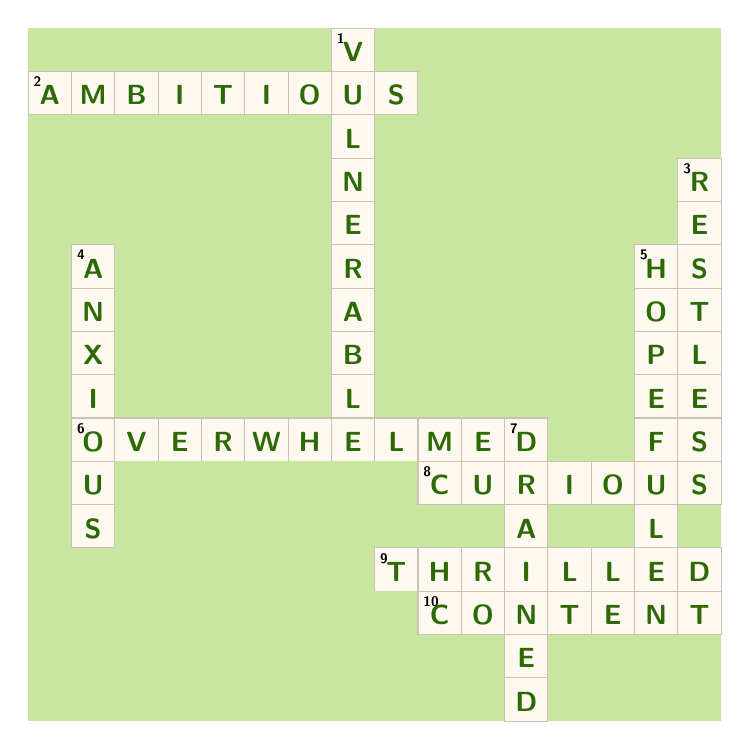
\begin{tikzpicture}[x=0.55cm,y=0.55cm]
\fill[deadcell] (0,0) rectangle (1,-1);
\fill[deadcell] (1,0) rectangle (2,-1);
\fill[deadcell] (2,0) rectangle (3,-1);
\fill[deadcell] (3,0) rectangle (4,-1);
\fill[deadcell] (4,0) rectangle (5,-1);
\fill[deadcell] (5,0) rectangle (6,-1);
\fill[deadcell] (6,0) rectangle (7,-1);
\fill[livecell] (7,0) rectangle (8,-1);
\draw[livecellborder] (7,0) rectangle (8,-1);
\node[anchor=north west,font=\tiny\bfseries,inner sep=1pt] at (7.05,-0.05) {1};
\node[font=\bfseries,color=cwletter] at (7.5,-0.55) {V};
\fill[deadcell] (8,0) rectangle (9,-1);
\fill[deadcell] (9,0) rectangle (10,-1);
\fill[deadcell] (10,0) rectangle (11,-1);
\fill[deadcell] (11,0) rectangle (12,-1);
\fill[deadcell] (12,0) rectangle (13,-1);
\fill[deadcell] (13,0) rectangle (14,-1);
\fill[deadcell] (14,0) rectangle (15,-1);
\fill[deadcell] (15,0) rectangle (16,-1);
\fill[livecell] (0,-1) rectangle (1,-2);
\draw[livecellborder] (0,-1) rectangle (1,-2);
\node[anchor=north west,font=\tiny\bfseries,inner sep=1pt] at (0.05,-1.05) {2};
\node[font=\bfseries,color=cwletter] at (0.5,-1.55) {A};
\fill[livecell] (1,-1) rectangle (2,-2);
\draw[livecellborder] (1,-1) rectangle (2,-2);
\node[font=\bfseries,color=cwletter] at (1.5,-1.55) {M};
\fill[livecell] (2,-1) rectangle (3,-2);
\draw[livecellborder] (2,-1) rectangle (3,-2);
\node[font=\bfseries,color=cwletter] at (2.5,-1.55) {B};
\fill[livecell] (3,-1) rectangle (4,-2);
\draw[livecellborder] (3,-1) rectangle (4,-2);
\node[font=\bfseries,color=cwletter] at (3.5,-1.55) {I};
\fill[livecell] (4,-1) rectangle (5,-2);
\draw[livecellborder] (4,-1) rectangle (5,-2);
\node[font=\bfseries,color=cwletter] at (4.5,-1.55) {T};
\fill[livecell] (5,-1) rectangle (6,-2);
\draw[livecellborder] (5,-1) rectangle (6,-2);
\node[font=\bfseries,color=cwletter] at (5.5,-1.55) {I};
\fill[livecell] (6,-1) rectangle (7,-2);
\draw[livecellborder] (6,-1) rectangle (7,-2);
\node[font=\bfseries,color=cwletter] at (6.5,-1.55) {O};
\fill[livecell] (7,-1) rectangle (8,-2);
\draw[livecellborder] (7,-1) rectangle (8,-2);
\node[font=\bfseries,color=cwletter] at (7.5,-1.55) {U};
\fill[livecell] (8,-1) rectangle (9,-2);
\draw[livecellborder] (8,-1) rectangle (9,-2);
\node[font=\bfseries,color=cwletter] at (8.5,-1.55) {S};
\fill[deadcell] (9,-1) rectangle (10,-2);
\fill[deadcell] (10,-1) rectangle (11,-2);
\fill[deadcell] (11,-1) rectangle (12,-2);
\fill[deadcell] (12,-1) rectangle (13,-2);
\fill[deadcell] (13,-1) rectangle (14,-2);
\fill[deadcell] (14,-1) rectangle (15,-2);
\fill[deadcell] (15,-1) rectangle (16,-2);
\fill[deadcell] (0,-2) rectangle (1,-3);
\fill[deadcell] (1,-2) rectangle (2,-3);
\fill[deadcell] (2,-2) rectangle (3,-3);
\fill[deadcell] (3,-2) rectangle (4,-3);
\fill[deadcell] (4,-2) rectangle (5,-3);
\fill[deadcell] (5,-2) rectangle (6,-3);
\fill[deadcell] (6,-2) rectangle (7,-3);
\fill[livecell] (7,-2) rectangle (8,-3);
\draw[livecellborder] (7,-2) rectangle (8,-3);
\node[font=\bfseries,color=cwletter] at (7.5,-2.55) {L};
\fill[deadcell] (8,-2) rectangle (9,-3);
\fill[deadcell] (9,-2) rectangle (10,-3);
\fill[deadcell] (10,-2) rectangle (11,-3);
\fill[deadcell] (11,-2) rectangle (12,-3);
\fill[deadcell] (12,-2) rectangle (13,-3);
\fill[deadcell] (13,-2) rectangle (14,-3);
\fill[deadcell] (14,-2) rectangle (15,-3);
\fill[deadcell] (15,-2) rectangle (16,-3);
\fill[deadcell] (0,-3) rectangle (1,-4);
\fill[deadcell] (1,-3) rectangle (2,-4);
\fill[deadcell] (2,-3) rectangle (3,-4);
\fill[deadcell] (3,-3) rectangle (4,-4);
\fill[deadcell] (4,-3) rectangle (5,-4);
\fill[deadcell] (5,-3) rectangle (6,-4);
\fill[deadcell] (6,-3) rectangle (7,-4);
\fill[livecell] (7,-3) rectangle (8,-4);
\draw[livecellborder] (7,-3) rectangle (8,-4);
\node[font=\bfseries,color=cwletter] at (7.5,-3.55) {N};
\fill[deadcell] (8,-3) rectangle (9,-4);
\fill[deadcell] (9,-3) rectangle (10,-4);
\fill[deadcell] (10,-3) rectangle (11,-4);
\fill[deadcell] (11,-3) rectangle (12,-4);
\fill[deadcell] (12,-3) rectangle (13,-4);
\fill[deadcell] (13,-3) rectangle (14,-4);
\fill[deadcell] (14,-3) rectangle (15,-4);
\fill[livecell] (15,-3) rectangle (16,-4);
\draw[livecellborder] (15,-3) rectangle (16,-4);
\node[anchor=north west,font=\tiny\bfseries,inner sep=1pt] at (15.05,-3.05) {3};
\node[font=\bfseries,color=cwletter] at (15.5,-3.55) {R};
\fill[deadcell] (0,-4) rectangle (1,-5);
\fill[deadcell] (1,-4) rectangle (2,-5);
\fill[deadcell] (2,-4) rectangle (3,-5);
\fill[deadcell] (3,-4) rectangle (4,-5);
\fill[deadcell] (4,-4) rectangle (5,-5);
\fill[deadcell] (5,-4) rectangle (6,-5);
\fill[deadcell] (6,-4) rectangle (7,-5);
\fill[livecell] (7,-4) rectangle (8,-5);
\draw[livecellborder] (7,-4) rectangle (8,-5);
\node[font=\bfseries,color=cwletter] at (7.5,-4.55) {E};
\fill[deadcell] (8,-4) rectangle (9,-5);
\fill[deadcell] (9,-4) rectangle (10,-5);
\fill[deadcell] (10,-4) rectangle (11,-5);
\fill[deadcell] (11,-4) rectangle (12,-5);
\fill[deadcell] (12,-4) rectangle (13,-5);
\fill[deadcell] (13,-4) rectangle (14,-5);
\fill[deadcell] (14,-4) rectangle (15,-5);
\fill[livecell] (15,-4) rectangle (16,-5);
\draw[livecellborder] (15,-4) rectangle (16,-5);
\node[font=\bfseries,color=cwletter] at (15.5,-4.55) {E};
\fill[deadcell] (0,-5) rectangle (1,-6);
\fill[livecell] (1,-5) rectangle (2,-6);
\draw[livecellborder] (1,-5) rectangle (2,-6);
\node[anchor=north west,font=\tiny\bfseries,inner sep=1pt] at (1.05,-5.05) {4};
\node[font=\bfseries,color=cwletter] at (1.5,-5.55) {A};
\fill[deadcell] (2,-5) rectangle (3,-6);
\fill[deadcell] (3,-5) rectangle (4,-6);
\fill[deadcell] (4,-5) rectangle (5,-6);
\fill[deadcell] (5,-5) rectangle (6,-6);
\fill[deadcell] (6,-5) rectangle (7,-6);
\fill[livecell] (7,-5) rectangle (8,-6);
\draw[livecellborder] (7,-5) rectangle (8,-6);
\node[font=\bfseries,color=cwletter] at (7.5,-5.55) {R};
\fill[deadcell] (8,-5) rectangle (9,-6);
\fill[deadcell] (9,-5) rectangle (10,-6);
\fill[deadcell] (10,-5) rectangle (11,-6);
\fill[deadcell] (11,-5) rectangle (12,-6);
\fill[deadcell] (12,-5) rectangle (13,-6);
\fill[deadcell] (13,-5) rectangle (14,-6);
\fill[livecell] (14,-5) rectangle (15,-6);
\draw[livecellborder] (14,-5) rectangle (15,-6);
\node[anchor=north west,font=\tiny\bfseries,inner sep=1pt] at (14.05,-5.05) {5};
\node[font=\bfseries,color=cwletter] at (14.5,-5.55) {H};
\fill[livecell] (15,-5) rectangle (16,-6);
\draw[livecellborder] (15,-5) rectangle (16,-6);
\node[font=\bfseries,color=cwletter] at (15.5,-5.55) {S};
\fill[deadcell] (0,-6) rectangle (1,-7);
\fill[livecell] (1,-6) rectangle (2,-7);
\draw[livecellborder] (1,-6) rectangle (2,-7);
\node[font=\bfseries,color=cwletter] at (1.5,-6.55) {N};
\fill[deadcell] (2,-6) rectangle (3,-7);
\fill[deadcell] (3,-6) rectangle (4,-7);
\fill[deadcell] (4,-6) rectangle (5,-7);
\fill[deadcell] (5,-6) rectangle (6,-7);
\fill[deadcell] (6,-6) rectangle (7,-7);
\fill[livecell] (7,-6) rectangle (8,-7);
\draw[livecellborder] (7,-6) rectangle (8,-7);
\node[font=\bfseries,color=cwletter] at (7.5,-6.55) {A};
\fill[deadcell] (8,-6) rectangle (9,-7);
\fill[deadcell] (9,-6) rectangle (10,-7);
\fill[deadcell] (10,-6) rectangle (11,-7);
\fill[deadcell] (11,-6) rectangle (12,-7);
\fill[deadcell] (12,-6) rectangle (13,-7);
\fill[deadcell] (13,-6) rectangle (14,-7);
\fill[livecell] (14,-6) rectangle (15,-7);
\draw[livecellborder] (14,-6) rectangle (15,-7);
\node[font=\bfseries,color=cwletter] at (14.5,-6.55) {O};
\fill[livecell] (15,-6) rectangle (16,-7);
\draw[livecellborder] (15,-6) rectangle (16,-7);
\node[font=\bfseries,color=cwletter] at (15.5,-6.55) {T};
\fill[deadcell] (0,-7) rectangle (1,-8);
\fill[livecell] (1,-7) rectangle (2,-8);
\draw[livecellborder] (1,-7) rectangle (2,-8);
\node[font=\bfseries,color=cwletter] at (1.5,-7.55) {X};
\fill[deadcell] (2,-7) rectangle (3,-8);
\fill[deadcell] (3,-7) rectangle (4,-8);
\fill[deadcell] (4,-7) rectangle (5,-8);
\fill[deadcell] (5,-7) rectangle (6,-8);
\fill[deadcell] (6,-7) rectangle (7,-8);
\fill[livecell] (7,-7) rectangle (8,-8);
\draw[livecellborder] (7,-7) rectangle (8,-8);
\node[font=\bfseries,color=cwletter] at (7.5,-7.55) {B};
\fill[deadcell] (8,-7) rectangle (9,-8);
\fill[deadcell] (9,-7) rectangle (10,-8);
\fill[deadcell] (10,-7) rectangle (11,-8);
\fill[deadcell] (11,-7) rectangle (12,-8);
\fill[deadcell] (12,-7) rectangle (13,-8);
\fill[deadcell] (13,-7) rectangle (14,-8);
\fill[livecell] (14,-7) rectangle (15,-8);
\draw[livecellborder] (14,-7) rectangle (15,-8);
\node[font=\bfseries,color=cwletter] at (14.5,-7.55) {P};
\fill[livecell] (15,-7) rectangle (16,-8);
\draw[livecellborder] (15,-7) rectangle (16,-8);
\node[font=\bfseries,color=cwletter] at (15.5,-7.55) {L};
\fill[deadcell] (0,-8) rectangle (1,-9);
\fill[livecell] (1,-8) rectangle (2,-9);
\draw[livecellborder] (1,-8) rectangle (2,-9);
\node[font=\bfseries,color=cwletter] at (1.5,-8.55) {I};
\fill[deadcell] (2,-8) rectangle (3,-9);
\fill[deadcell] (3,-8) rectangle (4,-9);
\fill[deadcell] (4,-8) rectangle (5,-9);
\fill[deadcell] (5,-8) rectangle (6,-9);
\fill[deadcell] (6,-8) rectangle (7,-9);
\fill[livecell] (7,-8) rectangle (8,-9);
\draw[livecellborder] (7,-8) rectangle (8,-9);
\node[font=\bfseries,color=cwletter] at (7.5,-8.55) {L};
\fill[deadcell] (8,-8) rectangle (9,-9);
\fill[deadcell] (9,-8) rectangle (10,-9);
\fill[deadcell] (10,-8) rectangle (11,-9);
\fill[deadcell] (11,-8) rectangle (12,-9);
\fill[deadcell] (12,-8) rectangle (13,-9);
\fill[deadcell] (13,-8) rectangle (14,-9);
\fill[livecell] (14,-8) rectangle (15,-9);
\draw[livecellborder] (14,-8) rectangle (15,-9);
\node[font=\bfseries,color=cwletter] at (14.5,-8.55) {E};
\fill[livecell] (15,-8) rectangle (16,-9);
\draw[livecellborder] (15,-8) rectangle (16,-9);
\node[font=\bfseries,color=cwletter] at (15.5,-8.55) {E};
\fill[deadcell] (0,-9) rectangle (1,-10);
\fill[livecell] (1,-9) rectangle (2,-10);
\draw[livecellborder] (1,-9) rectangle (2,-10);
\node[anchor=north west,font=\tiny\bfseries,inner sep=1pt] at (1.05,-9.05) {6};
\node[font=\bfseries,color=cwletter] at (1.5,-9.55) {O};
\fill[livecell] (2,-9) rectangle (3,-10);
\draw[livecellborder] (2,-9) rectangle (3,-10);
\node[font=\bfseries,color=cwletter] at (2.5,-9.55) {V};
\fill[livecell] (3,-9) rectangle (4,-10);
\draw[livecellborder] (3,-9) rectangle (4,-10);
\node[font=\bfseries,color=cwletter] at (3.5,-9.55) {E};
\fill[livecell] (4,-9) rectangle (5,-10);
\draw[livecellborder] (4,-9) rectangle (5,-10);
\node[font=\bfseries,color=cwletter] at (4.5,-9.55) {R};
\fill[livecell] (5,-9) rectangle (6,-10);
\draw[livecellborder] (5,-9) rectangle (6,-10);
\node[font=\bfseries,color=cwletter] at (5.5,-9.55) {W};
\fill[livecell] (6,-9) rectangle (7,-10);
\draw[livecellborder] (6,-9) rectangle (7,-10);
\node[font=\bfseries,color=cwletter] at (6.5,-9.55) {H};
\fill[livecell] (7,-9) rectangle (8,-10);
\draw[livecellborder] (7,-9) rectangle (8,-10);
\node[font=\bfseries,color=cwletter] at (7.5,-9.55) {E};
\fill[livecell] (8,-9) rectangle (9,-10);
\draw[livecellborder] (8,-9) rectangle (9,-10);
\node[font=\bfseries,color=cwletter] at (8.5,-9.55) {L};
\fill[livecell] (9,-9) rectangle (10,-10);
\draw[livecellborder] (9,-9) rectangle (10,-10);
\node[font=\bfseries,color=cwletter] at (9.5,-9.55) {M};
\fill[livecell] (10,-9) rectangle (11,-10);
\draw[livecellborder] (10,-9) rectangle (11,-10);
\node[font=\bfseries,color=cwletter] at (10.5,-9.55) {E};
\fill[livecell] (11,-9) rectangle (12,-10);
\draw[livecellborder] (11,-9) rectangle (12,-10);
\node[anchor=north west,font=\tiny\bfseries,inner sep=1pt] at (11.05,-9.05) {7};
\node[font=\bfseries,color=cwletter] at (11.5,-9.55) {D};
\fill[deadcell] (12,-9) rectangle (13,-10);
\fill[deadcell] (13,-9) rectangle (14,-10);
\fill[livecell] (14,-9) rectangle (15,-10);
\draw[livecellborder] (14,-9) rectangle (15,-10);
\node[font=\bfseries,color=cwletter] at (14.5,-9.55) {F};
\fill[livecell] (15,-9) rectangle (16,-10);
\draw[livecellborder] (15,-9) rectangle (16,-10);
\node[font=\bfseries,color=cwletter] at (15.5,-9.55) {S};
\fill[deadcell] (0,-10) rectangle (1,-11);
\fill[livecell] (1,-10) rectangle (2,-11);
\draw[livecellborder] (1,-10) rectangle (2,-11);
\node[font=\bfseries,color=cwletter] at (1.5,-10.55) {U};
\fill[deadcell] (2,-10) rectangle (3,-11);
\fill[deadcell] (3,-10) rectangle (4,-11);
\fill[deadcell] (4,-10) rectangle (5,-11);
\fill[deadcell] (5,-10) rectangle (6,-11);
\fill[deadcell] (6,-10) rectangle (7,-11);
\fill[deadcell] (7,-10) rectangle (8,-11);
\fill[deadcell] (8,-10) rectangle (9,-11);
\fill[livecell] (9,-10) rectangle (10,-11);
\draw[livecellborder] (9,-10) rectangle (10,-11);
\node[anchor=north west,font=\tiny\bfseries,inner sep=1pt] at (9.05,-10.05) {8};
\node[font=\bfseries,color=cwletter] at (9.5,-10.55) {C};
\fill[livecell] (10,-10) rectangle (11,-11);
\draw[livecellborder] (10,-10) rectangle (11,-11);
\node[font=\bfseries,color=cwletter] at (10.5,-10.55) {U};
\fill[livecell] (11,-10) rectangle (12,-11);
\draw[livecellborder] (11,-10) rectangle (12,-11);
\node[font=\bfseries,color=cwletter] at (11.5,-10.55) {R};
\fill[livecell] (12,-10) rectangle (13,-11);
\draw[livecellborder] (12,-10) rectangle (13,-11);
\node[font=\bfseries,color=cwletter] at (12.5,-10.55) {I};
\fill[livecell] (13,-10) rectangle (14,-11);
\draw[livecellborder] (13,-10) rectangle (14,-11);
\node[font=\bfseries,color=cwletter] at (13.5,-10.55) {O};
\fill[livecell] (14,-10) rectangle (15,-11);
\draw[livecellborder] (14,-10) rectangle (15,-11);
\node[font=\bfseries,color=cwletter] at (14.5,-10.55) {U};
\fill[livecell] (15,-10) rectangle (16,-11);
\draw[livecellborder] (15,-10) rectangle (16,-11);
\node[font=\bfseries,color=cwletter] at (15.5,-10.55) {S};
\fill[deadcell] (0,-11) rectangle (1,-12);
\fill[livecell] (1,-11) rectangle (2,-12);
\draw[livecellborder] (1,-11) rectangle (2,-12);
\node[font=\bfseries,color=cwletter] at (1.5,-11.55) {S};
\fill[deadcell] (2,-11) rectangle (3,-12);
\fill[deadcell] (3,-11) rectangle (4,-12);
\fill[deadcell] (4,-11) rectangle (5,-12);
\fill[deadcell] (5,-11) rectangle (6,-12);
\fill[deadcell] (6,-11) rectangle (7,-12);
\fill[deadcell] (7,-11) rectangle (8,-12);
\fill[deadcell] (8,-11) rectangle (9,-12);
\fill[deadcell] (9,-11) rectangle (10,-12);
\fill[deadcell] (10,-11) rectangle (11,-12);
\fill[livecell] (11,-11) rectangle (12,-12);
\draw[livecellborder] (11,-11) rectangle (12,-12);
\node[font=\bfseries,color=cwletter] at (11.5,-11.55) {A};
\fill[deadcell] (12,-11) rectangle (13,-12);
\fill[deadcell] (13,-11) rectangle (14,-12);
\fill[livecell] (14,-11) rectangle (15,-12);
\draw[livecellborder] (14,-11) rectangle (15,-12);
\node[font=\bfseries,color=cwletter] at (14.5,-11.55) {L};
\fill[deadcell] (15,-11) rectangle (16,-12);
\fill[deadcell] (0,-12) rectangle (1,-13);
\fill[deadcell] (1,-12) rectangle (2,-13);
\fill[deadcell] (2,-12) rectangle (3,-13);
\fill[deadcell] (3,-12) rectangle (4,-13);
\fill[deadcell] (4,-12) rectangle (5,-13);
\fill[deadcell] (5,-12) rectangle (6,-13);
\fill[deadcell] (6,-12) rectangle (7,-13);
\fill[deadcell] (7,-12) rectangle (8,-13);
\fill[livecell] (8,-12) rectangle (9,-13);
\draw[livecellborder] (8,-12) rectangle (9,-13);
\node[anchor=north west,font=\tiny\bfseries,inner sep=1pt] at (8.05,-12.05) {9};
\node[font=\bfseries,color=cwletter] at (8.5,-12.55) {T};
\fill[livecell] (9,-12) rectangle (10,-13);
\draw[livecellborder] (9,-12) rectangle (10,-13);
\node[font=\bfseries,color=cwletter] at (9.5,-12.55) {H};
\fill[livecell] (10,-12) rectangle (11,-13);
\draw[livecellborder] (10,-12) rectangle (11,-13);
\node[font=\bfseries,color=cwletter] at (10.5,-12.55) {R};
\fill[livecell] (11,-12) rectangle (12,-13);
\draw[livecellborder] (11,-12) rectangle (12,-13);
\node[font=\bfseries,color=cwletter] at (11.5,-12.55) {I};
\fill[livecell] (12,-12) rectangle (13,-13);
\draw[livecellborder] (12,-12) rectangle (13,-13);
\node[font=\bfseries,color=cwletter] at (12.5,-12.55) {L};
\fill[livecell] (13,-12) rectangle (14,-13);
\draw[livecellborder] (13,-12) rectangle (14,-13);
\node[font=\bfseries,color=cwletter] at (13.5,-12.55) {L};
\fill[livecell] (14,-12) rectangle (15,-13);
\draw[livecellborder] (14,-12) rectangle (15,-13);
\node[font=\bfseries,color=cwletter] at (14.5,-12.55) {E};
\fill[livecell] (15,-12) rectangle (16,-13);
\draw[livecellborder] (15,-12) rectangle (16,-13);
\node[font=\bfseries,color=cwletter] at (15.5,-12.55) {D};
\fill[deadcell] (0,-13) rectangle (1,-14);
\fill[deadcell] (1,-13) rectangle (2,-14);
\fill[deadcell] (2,-13) rectangle (3,-14);
\fill[deadcell] (3,-13) rectangle (4,-14);
\fill[deadcell] (4,-13) rectangle (5,-14);
\fill[deadcell] (5,-13) rectangle (6,-14);
\fill[deadcell] (6,-13) rectangle (7,-14);
\fill[deadcell] (7,-13) rectangle (8,-14);
\fill[deadcell] (8,-13) rectangle (9,-14);
\fill[livecell] (9,-13) rectangle (10,-14);
\draw[livecellborder] (9,-13) rectangle (10,-14);
\node[anchor=north west,font=\tiny\bfseries,inner sep=1pt] at (9.05,-13.05) {10};
\node[font=\bfseries,color=cwletter] at (9.5,-13.55) {C};
\fill[livecell] (10,-13) rectangle (11,-14);
\draw[livecellborder] (10,-13) rectangle (11,-14);
\node[font=\bfseries,color=cwletter] at (10.5,-13.55) {O};
\fill[livecell] (11,-13) rectangle (12,-14);
\draw[livecellborder] (11,-13) rectangle (12,-14);
\node[font=\bfseries,color=cwletter] at (11.5,-13.55) {N};
\fill[livecell] (12,-13) rectangle (13,-14);
\draw[livecellborder] (12,-13) rectangle (13,-14);
\node[font=\bfseries,color=cwletter] at (12.5,-13.55) {T};
\fill[livecell] (13,-13) rectangle (14,-14);
\draw[livecellborder] (13,-13) rectangle (14,-14);
\node[font=\bfseries,color=cwletter] at (13.5,-13.55) {E};
\fill[livecell] (14,-13) rectangle (15,-14);
\draw[livecellborder] (14,-13) rectangle (15,-14);
\node[font=\bfseries,color=cwletter] at (14.5,-13.55) {N};
\fill[livecell] (15,-13) rectangle (16,-14);
\draw[livecellborder] (15,-13) rectangle (16,-14);
\node[font=\bfseries,color=cwletter] at (15.5,-13.55) {T};
\fill[deadcell] (0,-14) rectangle (1,-15);
\fill[deadcell] (1,-14) rectangle (2,-15);
\fill[deadcell] (2,-14) rectangle (3,-15);
\fill[deadcell] (3,-14) rectangle (4,-15);
\fill[deadcell] (4,-14) rectangle (5,-15);
\fill[deadcell] (5,-14) rectangle (6,-15);
\fill[deadcell] (6,-14) rectangle (7,-15);
\fill[deadcell] (7,-14) rectangle (8,-15);
\fill[deadcell] (8,-14) rectangle (9,-15);
\fill[deadcell] (9,-14) rectangle (10,-15);
\fill[deadcell] (10,-14) rectangle (11,-15);
\fill[livecell] (11,-14) rectangle (12,-15);
\draw[livecellborder] (11,-14) rectangle (12,-15);
\node[font=\bfseries,color=cwletter] at (11.5,-14.55) {E};
\fill[deadcell] (12,-14) rectangle (13,-15);
\fill[deadcell] (13,-14) rectangle (14,-15);
\fill[deadcell] (14,-14) rectangle (15,-15);
\fill[deadcell] (15,-14) rectangle (16,-15);
\fill[deadcell] (0,-15) rectangle (1,-16);
\fill[deadcell] (1,-15) rectangle (2,-16);
\fill[deadcell] (2,-15) rectangle (3,-16);
\fill[deadcell] (3,-15) rectangle (4,-16);
\fill[deadcell] (4,-15) rectangle (5,-16);
\fill[deadcell] (5,-15) rectangle (6,-16);
\fill[deadcell] (6,-15) rectangle (7,-16);
\fill[deadcell] (7,-15) rectangle (8,-16);
\fill[deadcell] (8,-15) rectangle (9,-16);
\fill[deadcell] (9,-15) rectangle (10,-16);
\fill[deadcell] (10,-15) rectangle (11,-16);
\fill[livecell] (11,-15) rectangle (12,-16);
\draw[livecellborder] (11,-15) rectangle (12,-16);
\node[font=\bfseries,color=cwletter] at (11.5,-15.55) {D};
\fill[deadcell] (12,-15) rectangle (13,-16);
\fill[deadcell] (13,-15) rectangle (14,-16);
\fill[deadcell] (14,-15) rectangle (15,-16);
\fill[deadcell] (15,-15) rectangle (16,-16);
\end{tikzpicture}
\end{center}

\newpage
\section*{}\sectionmark{Teacher key — Wordsearch}
\sectionhead{K7}{tyextras}{Wordsearch key}{}{}
\begin{center}
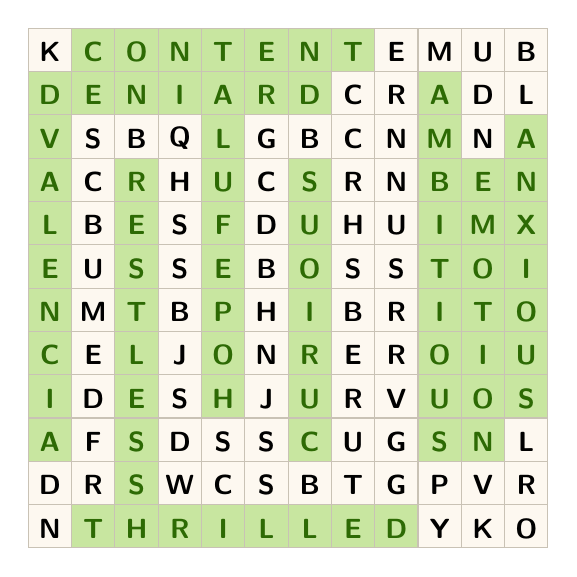
\begin{tikzpicture}[x=0.55cm,y=0.55cm]
\fill[livecell] (0,0) rectangle (1,-1);
\draw[livecellborder] (0,0) rectangle (1,-1);
\node[font=\bfseries] at (0.5,-0.55) {K};
\fill[ansgreen] (1,0) rectangle (2,-1);
\draw[livecellborder] (1,0) rectangle (2,-1);
\node[font=\bfseries,color=ansgreendark] at (1.5,-0.55) {C};
\fill[ansgreen] (2,0) rectangle (3,-1);
\draw[livecellborder] (2,0) rectangle (3,-1);
\node[font=\bfseries,color=ansgreendark] at (2.5,-0.55) {O};
\fill[ansgreen] (3,0) rectangle (4,-1);
\draw[livecellborder] (3,0) rectangle (4,-1);
\node[font=\bfseries,color=ansgreendark] at (3.5,-0.55) {N};
\fill[ansgreen] (4,0) rectangle (5,-1);
\draw[livecellborder] (4,0) rectangle (5,-1);
\node[font=\bfseries,color=ansgreendark] at (4.5,-0.55) {T};
\fill[ansgreen] (5,0) rectangle (6,-1);
\draw[livecellborder] (5,0) rectangle (6,-1);
\node[font=\bfseries,color=ansgreendark] at (5.5,-0.55) {E};
\fill[ansgreen] (6,0) rectangle (7,-1);
\draw[livecellborder] (6,0) rectangle (7,-1);
\node[font=\bfseries,color=ansgreendark] at (6.5,-0.55) {N};
\fill[ansgreen] (7,0) rectangle (8,-1);
\draw[livecellborder] (7,0) rectangle (8,-1);
\node[font=\bfseries,color=ansgreendark] at (7.5,-0.55) {T};
\fill[livecell] (8,0) rectangle (9,-1);
\draw[livecellborder] (8,0) rectangle (9,-1);
\node[font=\bfseries] at (8.5,-0.55) {E};
\fill[livecell] (9,0) rectangle (10,-1);
\draw[livecellborder] (9,0) rectangle (10,-1);
\node[font=\bfseries] at (9.5,-0.55) {M};
\fill[livecell] (10,0) rectangle (11,-1);
\draw[livecellborder] (10,0) rectangle (11,-1);
\node[font=\bfseries] at (10.5,-0.55) {U};
\fill[livecell] (11,0) rectangle (12,-1);
\draw[livecellborder] (11,0) rectangle (12,-1);
\node[font=\bfseries] at (11.5,-0.55) {B};
\fill[ansgreen] (0,-1) rectangle (1,-2);
\draw[livecellborder] (0,-1) rectangle (1,-2);
\node[font=\bfseries,color=ansgreendark] at (0.5,-1.55) {D};
\fill[ansgreen] (1,-1) rectangle (2,-2);
\draw[livecellborder] (1,-1) rectangle (2,-2);
\node[font=\bfseries,color=ansgreendark] at (1.5,-1.55) {E};
\fill[ansgreen] (2,-1) rectangle (3,-2);
\draw[livecellborder] (2,-1) rectangle (3,-2);
\node[font=\bfseries,color=ansgreendark] at (2.5,-1.55) {N};
\fill[ansgreen] (3,-1) rectangle (4,-2);
\draw[livecellborder] (3,-1) rectangle (4,-2);
\node[font=\bfseries,color=ansgreendark] at (3.5,-1.55) {I};
\fill[ansgreen] (4,-1) rectangle (5,-2);
\draw[livecellborder] (4,-1) rectangle (5,-2);
\node[font=\bfseries,color=ansgreendark] at (4.5,-1.55) {A};
\fill[ansgreen] (5,-1) rectangle (6,-2);
\draw[livecellborder] (5,-1) rectangle (6,-2);
\node[font=\bfseries,color=ansgreendark] at (5.5,-1.55) {R};
\fill[ansgreen] (6,-1) rectangle (7,-2);
\draw[livecellborder] (6,-1) rectangle (7,-2);
\node[font=\bfseries,color=ansgreendark] at (6.5,-1.55) {D};
\fill[livecell] (7,-1) rectangle (8,-2);
\draw[livecellborder] (7,-1) rectangle (8,-2);
\node[font=\bfseries] at (7.5,-1.55) {C};
\fill[livecell] (8,-1) rectangle (9,-2);
\draw[livecellborder] (8,-1) rectangle (9,-2);
\node[font=\bfseries] at (8.5,-1.55) {R};
\fill[ansgreen] (9,-1) rectangle (10,-2);
\draw[livecellborder] (9,-1) rectangle (10,-2);
\node[font=\bfseries,color=ansgreendark] at (9.5,-1.55) {A};
\fill[livecell] (10,-1) rectangle (11,-2);
\draw[livecellborder] (10,-1) rectangle (11,-2);
\node[font=\bfseries] at (10.5,-1.55) {D};
\fill[livecell] (11,-1) rectangle (12,-2);
\draw[livecellborder] (11,-1) rectangle (12,-2);
\node[font=\bfseries] at (11.5,-1.55) {L};
\fill[ansgreen] (0,-2) rectangle (1,-3);
\draw[livecellborder] (0,-2) rectangle (1,-3);
\node[font=\bfseries,color=ansgreendark] at (0.5,-2.55) {V};
\fill[livecell] (1,-2) rectangle (2,-3);
\draw[livecellborder] (1,-2) rectangle (2,-3);
\node[font=\bfseries] at (1.5,-2.55) {S};
\fill[livecell] (2,-2) rectangle (3,-3);
\draw[livecellborder] (2,-2) rectangle (3,-3);
\node[font=\bfseries] at (2.5,-2.55) {B};
\fill[livecell] (3,-2) rectangle (4,-3);
\draw[livecellborder] (3,-2) rectangle (4,-3);
\node[font=\bfseries] at (3.5,-2.55) {Q};
\fill[ansgreen] (4,-2) rectangle (5,-3);
\draw[livecellborder] (4,-2) rectangle (5,-3);
\node[font=\bfseries,color=ansgreendark] at (4.5,-2.55) {L};
\fill[livecell] (5,-2) rectangle (6,-3);
\draw[livecellborder] (5,-2) rectangle (6,-3);
\node[font=\bfseries] at (5.5,-2.55) {G};
\fill[livecell] (6,-2) rectangle (7,-3);
\draw[livecellborder] (6,-2) rectangle (7,-3);
\node[font=\bfseries] at (6.5,-2.55) {B};
\fill[livecell] (7,-2) rectangle (8,-3);
\draw[livecellborder] (7,-2) rectangle (8,-3);
\node[font=\bfseries] at (7.5,-2.55) {C};
\fill[livecell] (8,-2) rectangle (9,-3);
\draw[livecellborder] (8,-2) rectangle (9,-3);
\node[font=\bfseries] at (8.5,-2.55) {N};
\fill[ansgreen] (9,-2) rectangle (10,-3);
\draw[livecellborder] (9,-2) rectangle (10,-3);
\node[font=\bfseries,color=ansgreendark] at (9.5,-2.55) {M};
\fill[livecell] (10,-2) rectangle (11,-3);
\draw[livecellborder] (10,-2) rectangle (11,-3);
\node[font=\bfseries] at (10.5,-2.55) {N};
\fill[ansgreen] (11,-2) rectangle (12,-3);
\draw[livecellborder] (11,-2) rectangle (12,-3);
\node[font=\bfseries,color=ansgreendark] at (11.5,-2.55) {A};
\fill[ansgreen] (0,-3) rectangle (1,-4);
\draw[livecellborder] (0,-3) rectangle (1,-4);
\node[font=\bfseries,color=ansgreendark] at (0.5,-3.55) {A};
\fill[livecell] (1,-3) rectangle (2,-4);
\draw[livecellborder] (1,-3) rectangle (2,-4);
\node[font=\bfseries] at (1.5,-3.55) {C};
\fill[ansgreen] (2,-3) rectangle (3,-4);
\draw[livecellborder] (2,-3) rectangle (3,-4);
\node[font=\bfseries,color=ansgreendark] at (2.5,-3.55) {R};
\fill[livecell] (3,-3) rectangle (4,-4);
\draw[livecellborder] (3,-3) rectangle (4,-4);
\node[font=\bfseries] at (3.5,-3.55) {H};
\fill[ansgreen] (4,-3) rectangle (5,-4);
\draw[livecellborder] (4,-3) rectangle (5,-4);
\node[font=\bfseries,color=ansgreendark] at (4.5,-3.55) {U};
\fill[livecell] (5,-3) rectangle (6,-4);
\draw[livecellborder] (5,-3) rectangle (6,-4);
\node[font=\bfseries] at (5.5,-3.55) {C};
\fill[ansgreen] (6,-3) rectangle (7,-4);
\draw[livecellborder] (6,-3) rectangle (7,-4);
\node[font=\bfseries,color=ansgreendark] at (6.5,-3.55) {S};
\fill[livecell] (7,-3) rectangle (8,-4);
\draw[livecellborder] (7,-3) rectangle (8,-4);
\node[font=\bfseries] at (7.5,-3.55) {R};
\fill[livecell] (8,-3) rectangle (9,-4);
\draw[livecellborder] (8,-3) rectangle (9,-4);
\node[font=\bfseries] at (8.5,-3.55) {N};
\fill[ansgreen] (9,-3) rectangle (10,-4);
\draw[livecellborder] (9,-3) rectangle (10,-4);
\node[font=\bfseries,color=ansgreendark] at (9.5,-3.55) {B};
\fill[ansgreen] (10,-3) rectangle (11,-4);
\draw[livecellborder] (10,-3) rectangle (11,-4);
\node[font=\bfseries,color=ansgreendark] at (10.5,-3.55) {E};
\fill[ansgreen] (11,-3) rectangle (12,-4);
\draw[livecellborder] (11,-3) rectangle (12,-4);
\node[font=\bfseries,color=ansgreendark] at (11.5,-3.55) {N};
\fill[ansgreen] (0,-4) rectangle (1,-5);
\draw[livecellborder] (0,-4) rectangle (1,-5);
\node[font=\bfseries,color=ansgreendark] at (0.5,-4.55) {L};
\fill[livecell] (1,-4) rectangle (2,-5);
\draw[livecellborder] (1,-4) rectangle (2,-5);
\node[font=\bfseries] at (1.5,-4.55) {B};
\fill[ansgreen] (2,-4) rectangle (3,-5);
\draw[livecellborder] (2,-4) rectangle (3,-5);
\node[font=\bfseries,color=ansgreendark] at (2.5,-4.55) {E};
\fill[livecell] (3,-4) rectangle (4,-5);
\draw[livecellborder] (3,-4) rectangle (4,-5);
\node[font=\bfseries] at (3.5,-4.55) {S};
\fill[ansgreen] (4,-4) rectangle (5,-5);
\draw[livecellborder] (4,-4) rectangle (5,-5);
\node[font=\bfseries,color=ansgreendark] at (4.5,-4.55) {F};
\fill[livecell] (5,-4) rectangle (6,-5);
\draw[livecellborder] (5,-4) rectangle (6,-5);
\node[font=\bfseries] at (5.5,-4.55) {D};
\fill[ansgreen] (6,-4) rectangle (7,-5);
\draw[livecellborder] (6,-4) rectangle (7,-5);
\node[font=\bfseries,color=ansgreendark] at (6.5,-4.55) {U};
\fill[livecell] (7,-4) rectangle (8,-5);
\draw[livecellborder] (7,-4) rectangle (8,-5);
\node[font=\bfseries] at (7.5,-4.55) {H};
\fill[livecell] (8,-4) rectangle (9,-5);
\draw[livecellborder] (8,-4) rectangle (9,-5);
\node[font=\bfseries] at (8.5,-4.55) {U};
\fill[ansgreen] (9,-4) rectangle (10,-5);
\draw[livecellborder] (9,-4) rectangle (10,-5);
\node[font=\bfseries,color=ansgreendark] at (9.5,-4.55) {I};
\fill[ansgreen] (10,-4) rectangle (11,-5);
\draw[livecellborder] (10,-4) rectangle (11,-5);
\node[font=\bfseries,color=ansgreendark] at (10.5,-4.55) {M};
\fill[ansgreen] (11,-4) rectangle (12,-5);
\draw[livecellborder] (11,-4) rectangle (12,-5);
\node[font=\bfseries,color=ansgreendark] at (11.5,-4.55) {X};
\fill[ansgreen] (0,-5) rectangle (1,-6);
\draw[livecellborder] (0,-5) rectangle (1,-6);
\node[font=\bfseries,color=ansgreendark] at (0.5,-5.55) {E};
\fill[livecell] (1,-5) rectangle (2,-6);
\draw[livecellborder] (1,-5) rectangle (2,-6);
\node[font=\bfseries] at (1.5,-5.55) {U};
\fill[ansgreen] (2,-5) rectangle (3,-6);
\draw[livecellborder] (2,-5) rectangle (3,-6);
\node[font=\bfseries,color=ansgreendark] at (2.5,-5.55) {S};
\fill[livecell] (3,-5) rectangle (4,-6);
\draw[livecellborder] (3,-5) rectangle (4,-6);
\node[font=\bfseries] at (3.5,-5.55) {S};
\fill[ansgreen] (4,-5) rectangle (5,-6);
\draw[livecellborder] (4,-5) rectangle (5,-6);
\node[font=\bfseries,color=ansgreendark] at (4.5,-5.55) {E};
\fill[livecell] (5,-5) rectangle (6,-6);
\draw[livecellborder] (5,-5) rectangle (6,-6);
\node[font=\bfseries] at (5.5,-5.55) {B};
\fill[ansgreen] (6,-5) rectangle (7,-6);
\draw[livecellborder] (6,-5) rectangle (7,-6);
\node[font=\bfseries,color=ansgreendark] at (6.5,-5.55) {O};
\fill[livecell] (7,-5) rectangle (8,-6);
\draw[livecellborder] (7,-5) rectangle (8,-6);
\node[font=\bfseries] at (7.5,-5.55) {S};
\fill[livecell] (8,-5) rectangle (9,-6);
\draw[livecellborder] (8,-5) rectangle (9,-6);
\node[font=\bfseries] at (8.5,-5.55) {S};
\fill[ansgreen] (9,-5) rectangle (10,-6);
\draw[livecellborder] (9,-5) rectangle (10,-6);
\node[font=\bfseries,color=ansgreendark] at (9.5,-5.55) {T};
\fill[ansgreen] (10,-5) rectangle (11,-6);
\draw[livecellborder] (10,-5) rectangle (11,-6);
\node[font=\bfseries,color=ansgreendark] at (10.5,-5.55) {O};
\fill[ansgreen] (11,-5) rectangle (12,-6);
\draw[livecellborder] (11,-5) rectangle (12,-6);
\node[font=\bfseries,color=ansgreendark] at (11.5,-5.55) {I};
\fill[ansgreen] (0,-6) rectangle (1,-7);
\draw[livecellborder] (0,-6) rectangle (1,-7);
\node[font=\bfseries,color=ansgreendark] at (0.5,-6.55) {N};
\fill[livecell] (1,-6) rectangle (2,-7);
\draw[livecellborder] (1,-6) rectangle (2,-7);
\node[font=\bfseries] at (1.5,-6.55) {M};
\fill[ansgreen] (2,-6) rectangle (3,-7);
\draw[livecellborder] (2,-6) rectangle (3,-7);
\node[font=\bfseries,color=ansgreendark] at (2.5,-6.55) {T};
\fill[livecell] (3,-6) rectangle (4,-7);
\draw[livecellborder] (3,-6) rectangle (4,-7);
\node[font=\bfseries] at (3.5,-6.55) {B};
\fill[ansgreen] (4,-6) rectangle (5,-7);
\draw[livecellborder] (4,-6) rectangle (5,-7);
\node[font=\bfseries,color=ansgreendark] at (4.5,-6.55) {P};
\fill[livecell] (5,-6) rectangle (6,-7);
\draw[livecellborder] (5,-6) rectangle (6,-7);
\node[font=\bfseries] at (5.5,-6.55) {H};
\fill[ansgreen] (6,-6) rectangle (7,-7);
\draw[livecellborder] (6,-6) rectangle (7,-7);
\node[font=\bfseries,color=ansgreendark] at (6.5,-6.55) {I};
\fill[livecell] (7,-6) rectangle (8,-7);
\draw[livecellborder] (7,-6) rectangle (8,-7);
\node[font=\bfseries] at (7.5,-6.55) {B};
\fill[livecell] (8,-6) rectangle (9,-7);
\draw[livecellborder] (8,-6) rectangle (9,-7);
\node[font=\bfseries] at (8.5,-6.55) {R};
\fill[ansgreen] (9,-6) rectangle (10,-7);
\draw[livecellborder] (9,-6) rectangle (10,-7);
\node[font=\bfseries,color=ansgreendark] at (9.5,-6.55) {I};
\fill[ansgreen] (10,-6) rectangle (11,-7);
\draw[livecellborder] (10,-6) rectangle (11,-7);
\node[font=\bfseries,color=ansgreendark] at (10.5,-6.55) {T};
\fill[ansgreen] (11,-6) rectangle (12,-7);
\draw[livecellborder] (11,-6) rectangle (12,-7);
\node[font=\bfseries,color=ansgreendark] at (11.5,-6.55) {O};
\fill[ansgreen] (0,-7) rectangle (1,-8);
\draw[livecellborder] (0,-7) rectangle (1,-8);
\node[font=\bfseries,color=ansgreendark] at (0.5,-7.55) {C};
\fill[livecell] (1,-7) rectangle (2,-8);
\draw[livecellborder] (1,-7) rectangle (2,-8);
\node[font=\bfseries] at (1.5,-7.55) {E};
\fill[ansgreen] (2,-7) rectangle (3,-8);
\draw[livecellborder] (2,-7) rectangle (3,-8);
\node[font=\bfseries,color=ansgreendark] at (2.5,-7.55) {L};
\fill[livecell] (3,-7) rectangle (4,-8);
\draw[livecellborder] (3,-7) rectangle (4,-8);
\node[font=\bfseries] at (3.5,-7.55) {J};
\fill[ansgreen] (4,-7) rectangle (5,-8);
\draw[livecellborder] (4,-7) rectangle (5,-8);
\node[font=\bfseries,color=ansgreendark] at (4.5,-7.55) {O};
\fill[livecell] (5,-7) rectangle (6,-8);
\draw[livecellborder] (5,-7) rectangle (6,-8);
\node[font=\bfseries] at (5.5,-7.55) {N};
\fill[ansgreen] (6,-7) rectangle (7,-8);
\draw[livecellborder] (6,-7) rectangle (7,-8);
\node[font=\bfseries,color=ansgreendark] at (6.5,-7.55) {R};
\fill[livecell] (7,-7) rectangle (8,-8);
\draw[livecellborder] (7,-7) rectangle (8,-8);
\node[font=\bfseries] at (7.5,-7.55) {E};
\fill[livecell] (8,-7) rectangle (9,-8);
\draw[livecellborder] (8,-7) rectangle (9,-8);
\node[font=\bfseries] at (8.5,-7.55) {R};
\fill[ansgreen] (9,-7) rectangle (10,-8);
\draw[livecellborder] (9,-7) rectangle (10,-8);
\node[font=\bfseries,color=ansgreendark] at (9.5,-7.55) {O};
\fill[ansgreen] (10,-7) rectangle (11,-8);
\draw[livecellborder] (10,-7) rectangle (11,-8);
\node[font=\bfseries,color=ansgreendark] at (10.5,-7.55) {I};
\fill[ansgreen] (11,-7) rectangle (12,-8);
\draw[livecellborder] (11,-7) rectangle (12,-8);
\node[font=\bfseries,color=ansgreendark] at (11.5,-7.55) {U};
\fill[ansgreen] (0,-8) rectangle (1,-9);
\draw[livecellborder] (0,-8) rectangle (1,-9);
\node[font=\bfseries,color=ansgreendark] at (0.5,-8.55) {I};
\fill[livecell] (1,-8) rectangle (2,-9);
\draw[livecellborder] (1,-8) rectangle (2,-9);
\node[font=\bfseries] at (1.5,-8.55) {D};
\fill[ansgreen] (2,-8) rectangle (3,-9);
\draw[livecellborder] (2,-8) rectangle (3,-9);
\node[font=\bfseries,color=ansgreendark] at (2.5,-8.55) {E};
\fill[livecell] (3,-8) rectangle (4,-9);
\draw[livecellborder] (3,-8) rectangle (4,-9);
\node[font=\bfseries] at (3.5,-8.55) {S};
\fill[ansgreen] (4,-8) rectangle (5,-9);
\draw[livecellborder] (4,-8) rectangle (5,-9);
\node[font=\bfseries,color=ansgreendark] at (4.5,-8.55) {H};
\fill[livecell] (5,-8) rectangle (6,-9);
\draw[livecellborder] (5,-8) rectangle (6,-9);
\node[font=\bfseries] at (5.5,-8.55) {J};
\fill[ansgreen] (6,-8) rectangle (7,-9);
\draw[livecellborder] (6,-8) rectangle (7,-9);
\node[font=\bfseries,color=ansgreendark] at (6.5,-8.55) {U};
\fill[livecell] (7,-8) rectangle (8,-9);
\draw[livecellborder] (7,-8) rectangle (8,-9);
\node[font=\bfseries] at (7.5,-8.55) {R};
\fill[livecell] (8,-8) rectangle (9,-9);
\draw[livecellborder] (8,-8) rectangle (9,-9);
\node[font=\bfseries] at (8.5,-8.55) {V};
\fill[ansgreen] (9,-8) rectangle (10,-9);
\draw[livecellborder] (9,-8) rectangle (10,-9);
\node[font=\bfseries,color=ansgreendark] at (9.5,-8.55) {U};
\fill[ansgreen] (10,-8) rectangle (11,-9);
\draw[livecellborder] (10,-8) rectangle (11,-9);
\node[font=\bfseries,color=ansgreendark] at (10.5,-8.55) {O};
\fill[ansgreen] (11,-8) rectangle (12,-9);
\draw[livecellborder] (11,-8) rectangle (12,-9);
\node[font=\bfseries,color=ansgreendark] at (11.5,-8.55) {S};
\fill[ansgreen] (0,-9) rectangle (1,-10);
\draw[livecellborder] (0,-9) rectangle (1,-10);
\node[font=\bfseries,color=ansgreendark] at (0.5,-9.55) {A};
\fill[livecell] (1,-9) rectangle (2,-10);
\draw[livecellborder] (1,-9) rectangle (2,-10);
\node[font=\bfseries] at (1.5,-9.55) {F};
\fill[ansgreen] (2,-9) rectangle (3,-10);
\draw[livecellborder] (2,-9) rectangle (3,-10);
\node[font=\bfseries,color=ansgreendark] at (2.5,-9.55) {S};
\fill[livecell] (3,-9) rectangle (4,-10);
\draw[livecellborder] (3,-9) rectangle (4,-10);
\node[font=\bfseries] at (3.5,-9.55) {D};
\fill[livecell] (4,-9) rectangle (5,-10);
\draw[livecellborder] (4,-9) rectangle (5,-10);
\node[font=\bfseries] at (4.5,-9.55) {S};
\fill[livecell] (5,-9) rectangle (6,-10);
\draw[livecellborder] (5,-9) rectangle (6,-10);
\node[font=\bfseries] at (5.5,-9.55) {S};
\fill[ansgreen] (6,-9) rectangle (7,-10);
\draw[livecellborder] (6,-9) rectangle (7,-10);
\node[font=\bfseries,color=ansgreendark] at (6.5,-9.55) {C};
\fill[livecell] (7,-9) rectangle (8,-10);
\draw[livecellborder] (7,-9) rectangle (8,-10);
\node[font=\bfseries] at (7.5,-9.55) {U};
\fill[livecell] (8,-9) rectangle (9,-10);
\draw[livecellborder] (8,-9) rectangle (9,-10);
\node[font=\bfseries] at (8.5,-9.55) {G};
\fill[ansgreen] (9,-9) rectangle (10,-10);
\draw[livecellborder] (9,-9) rectangle (10,-10);
\node[font=\bfseries,color=ansgreendark] at (9.5,-9.55) {S};
\fill[ansgreen] (10,-9) rectangle (11,-10);
\draw[livecellborder] (10,-9) rectangle (11,-10);
\node[font=\bfseries,color=ansgreendark] at (10.5,-9.55) {N};
\fill[livecell] (11,-9) rectangle (12,-10);
\draw[livecellborder] (11,-9) rectangle (12,-10);
\node[font=\bfseries] at (11.5,-9.55) {L};
\fill[livecell] (0,-10) rectangle (1,-11);
\draw[livecellborder] (0,-10) rectangle (1,-11);
\node[font=\bfseries] at (0.5,-10.55) {D};
\fill[livecell] (1,-10) rectangle (2,-11);
\draw[livecellborder] (1,-10) rectangle (2,-11);
\node[font=\bfseries] at (1.5,-10.55) {R};
\fill[ansgreen] (2,-10) rectangle (3,-11);
\draw[livecellborder] (2,-10) rectangle (3,-11);
\node[font=\bfseries,color=ansgreendark] at (2.5,-10.55) {S};
\fill[livecell] (3,-10) rectangle (4,-11);
\draw[livecellborder] (3,-10) rectangle (4,-11);
\node[font=\bfseries] at (3.5,-10.55) {W};
\fill[livecell] (4,-10) rectangle (5,-11);
\draw[livecellborder] (4,-10) rectangle (5,-11);
\node[font=\bfseries] at (4.5,-10.55) {C};
\fill[livecell] (5,-10) rectangle (6,-11);
\draw[livecellborder] (5,-10) rectangle (6,-11);
\node[font=\bfseries] at (5.5,-10.55) {S};
\fill[livecell] (6,-10) rectangle (7,-11);
\draw[livecellborder] (6,-10) rectangle (7,-11);
\node[font=\bfseries] at (6.5,-10.55) {B};
\fill[livecell] (7,-10) rectangle (8,-11);
\draw[livecellborder] (7,-10) rectangle (8,-11);
\node[font=\bfseries] at (7.5,-10.55) {T};
\fill[livecell] (8,-10) rectangle (9,-11);
\draw[livecellborder] (8,-10) rectangle (9,-11);
\node[font=\bfseries] at (8.5,-10.55) {G};
\fill[livecell] (9,-10) rectangle (10,-11);
\draw[livecellborder] (9,-10) rectangle (10,-11);
\node[font=\bfseries] at (9.5,-10.55) {P};
\fill[livecell] (10,-10) rectangle (11,-11);
\draw[livecellborder] (10,-10) rectangle (11,-11);
\node[font=\bfseries] at (10.5,-10.55) {V};
\fill[livecell] (11,-10) rectangle (12,-11);
\draw[livecellborder] (11,-10) rectangle (12,-11);
\node[font=\bfseries] at (11.5,-10.55) {R};
\fill[livecell] (0,-11) rectangle (1,-12);
\draw[livecellborder] (0,-11) rectangle (1,-12);
\node[font=\bfseries] at (0.5,-11.55) {N};
\fill[ansgreen] (1,-11) rectangle (2,-12);
\draw[livecellborder] (1,-11) rectangle (2,-12);
\node[font=\bfseries,color=ansgreendark] at (1.5,-11.55) {T};
\fill[ansgreen] (2,-11) rectangle (3,-12);
\draw[livecellborder] (2,-11) rectangle (3,-12);
\node[font=\bfseries,color=ansgreendark] at (2.5,-11.55) {H};
\fill[ansgreen] (3,-11) rectangle (4,-12);
\draw[livecellborder] (3,-11) rectangle (4,-12);
\node[font=\bfseries,color=ansgreendark] at (3.5,-11.55) {R};
\fill[ansgreen] (4,-11) rectangle (5,-12);
\draw[livecellborder] (4,-11) rectangle (5,-12);
\node[font=\bfseries,color=ansgreendark] at (4.5,-11.55) {I};
\fill[ansgreen] (5,-11) rectangle (6,-12);
\draw[livecellborder] (5,-11) rectangle (6,-12);
\node[font=\bfseries,color=ansgreendark] at (5.5,-11.55) {L};
\fill[ansgreen] (6,-11) rectangle (7,-12);
\draw[livecellborder] (6,-11) rectangle (7,-12);
\node[font=\bfseries,color=ansgreendark] at (6.5,-11.55) {L};
\fill[ansgreen] (7,-11) rectangle (8,-12);
\draw[livecellborder] (7,-11) rectangle (8,-12);
\node[font=\bfseries,color=ansgreendark] at (7.5,-11.55) {E};
\fill[ansgreen] (8,-11) rectangle (9,-12);
\draw[livecellborder] (8,-11) rectangle (9,-12);
\node[font=\bfseries,color=ansgreendark] at (8.5,-11.55) {D};
\fill[livecell] (9,-11) rectangle (10,-12);
\draw[livecellborder] (9,-11) rectangle (10,-12);
\node[font=\bfseries] at (9.5,-11.55) {Y};
\fill[livecell] (10,-11) rectangle (11,-12);
\draw[livecellborder] (10,-11) rectangle (11,-12);
\node[font=\bfseries] at (10.5,-11.55) {K};
\fill[livecell] (11,-11) rectangle (12,-12);
\draw[livecellborder] (11,-11) rectangle (12,-12);
\node[font=\bfseries] at (11.5,-11.55) {O};
\end{tikzpicture}
\end{center}
\vspace{6pt}
\begin{multicols}{2}
{\fontsize{12}{15}\selectfont
\textbf{1.} extremely excited and pleased~\textbf{\textcolor{ansgreendark}{— THRILLED}} \\[2pt]
\textbf{2.} believing things will turn out well~\textbf{\textcolor{ansgreendark}{— HOPEFUL}} \\[2pt]
\textbf{3.} wanting to know or learn more~\textbf{\textcolor{ansgreendark}{— CURIOUS}} \\[2pt]
\textbf{4.} unable to sit still or stop thinking~\textbf{\textcolor{ansgreendark}{— RESTLESS}} \\[2pt]
\textbf{5.} quietly happy with the way things are~\textbf{\textcolor{ansgreendark}{— CONTENT}} \\[2pt]
\columnbreak
\textbf{6.} completely without energy after effort~\textbf{\textcolor{ansgreendark}{— DRAINED}} \\[2pt]
\textbf{7.} wanting strongly to succeed in life~\textbf{\textcolor{ansgreendark}{— AMBITIOUS}} \\[2pt]
\textbf{8.} worried or nervous about something~\textbf{\textcolor{ansgreendark}{— ANXIOUS}} \\[2pt]
\textbf{9.} a strong feeling such as joy or fear~\textbf{\textcolor{ansgreendark}{— EMOTION}} \\[2pt]
\textbf{10.} the Spanish city where Aitana plays Roig Arena next spring~\textbf{\textcolor{ansgreendark}{— VALENCIA}} \\[2pt]
}
\end{multicols}

\sectionhead{K8}{tyextras}{Trackers updated}{}{}
\begin{itemize}[leftmargin=*]
  \item \textbf{False-friend tracker:} \texttt{sensible / sensible} marked USED. Worksheet: F1 18 Sept 2026.
  \item \textbf{Pronunciation tracker:} schwa /\textschwa/ in adjectives delivered as a custom drill (not from the canonical 17-exercise list — log under ``custom: F1 schwa adjectives'').
  \item \textbf{Phrasal-verb tracker:} \textit{cheer up} introduced. Top 2 senses: (1) make someone happier; (2) become happier.
\end{itemize}

\newpage
\section*{}\sectionmark{Teacher key — Pre-delivery check}
\sectionhead{K9}{tywriting}{Pre-delivery formatting check}{}{}
\begin{itemize}[leftmargin=*]
  \item Reading text 14pt~~$\checkmark$
  \item All other text $\geq$~12pt~~$\checkmark$
  \item No exercise split across pages~~$\checkmark$
  \item Logo on every page (header)~~$\checkmark$
  \item Valencia / Spain references woven in: Aitana, Roig Arena, L'Oceanogr\`afic, Malvarrosa, Albacete~~$\checkmark$
  \item Four mandatory extras present: short play · crossword · wordsearch · false-friend \& pronunciation drill~~$\checkmark$
\end{itemize}

\end{document}
